\documentclass[conference]{IEEEtran}
\IEEEoverridecommandlockouts
% The preceding line is only needed to identify funding in the first footnote. If that is unneeded, please comment it out.
\usepackage{cite}
\usepackage{amsmath,amssymb,amsfonts}
\usepackage{algorithmic}
\usepackage{graphicx}
\usepackage{listings}
\lstset{breaklines=true}
\usepackage{url}
\usepackage{hyperref}
\usepackage{dirtree}
\graphicspath{ {images/} }
\usepackage{textcomp}
\usepackage{xcolor}
\usepackage{todonotes}
\usepackage{subcaption}
\usepackage{placeins}
\usepackage{comment}

\usepackage{tikz}
\usetikzlibrary{calc, patterns, patterns.meta, shapes.geometric, arrows.meta, positioning, fit, decorations.pathreplacing, trees, arrows, shapes.misc, angles, quotes}
%Go-kart command \gokart{"x"}{"y"}{"rot_in_deg"}
\def\gokart#1#2#3{
    \begin{scope}[shift={(#1,#2)}, rotate=#3]
        \begin{scope}[shift={(0,-0.85)}] %Offset so (x,y) is the front bumper
            %Front bumper
            \draw[very thick] (-0.7, 0.75) -- (-0.5, 0.85) -- (0.5, 0.85) -- (0.7, 0.75);
            %Body
            \draw[fill=gray!30] (-0.5,-0.75) rectangle (0.5,0.75);
            %Wheels
            \draw[fill=black, rounded corners=0.75] (-0.6,0.6) rectangle (-0.4, 0.3); % Front left
            \draw[fill=black, rounded corners=0.75] (0.6,0.6) rectangle (0.4, 0.3); % Front right
            \draw[fill=black, rounded corners=0.75] (-0.6,-0.6) rectangle (-0.4, -0.3); % Rear left
            \draw[fill=black, rounded corners=0.75] (0.6,-0.6) rectangle (0.4, -0.3); % Rear right
            %Rear bumper
            \draw[very thick] (-0.6, -0.75) -- (-0.5, -0.8) -- (0.5, -0.8) -- (0.6, -0.75);
        \end{scope}
    \end{scope}
}


\usepackage{siunitx} 
\sisetup{locale = US}
\DeclareSIUnit{\Bit}{Bit}
\DeclareSIUnit{\baud}{Baud}
\DeclareSIUnit{\frame}{f}

\def\BibTeX{{\rm B\kern-.05em{\sc i\kern-.025em b}\kern-.08em
    T\kern-.1667em\lower.7ex\hbox{E}\kern-.125emX}}


\pagestyle{plain}

\begin{document}

\title{Development of a Radar-Based Emergency Braking System\\
{\large Leveraging mmWave Radar Sensor Technology for Object Detection}
}

\author{\IEEEauthorblockN{Luis Fernando Rodriguez Gutierrez}
\IEEEauthorblockA{\textit{Fachhochschule Dortmund} \\
\textit{M.Eng. Embedded Systems Engineering}\\
luis.rodriguez001@stud.fh-dortmund.de}

}


\maketitle


\begin{abstract}
The employment and integration of radar technologies for the implementation of odometry has recently emerged as a promissing alternative to traditional methods, which often rely on visual or LiDAR-based systems. 
Radar Technology is particularly advantageous due to its robustness in various environmental conditions, such as fog, rain, and dust, where other systems results may degrade.

This work focus in the estimation of the vehicle's ego-motion using a single mmWave radar sensor which is mounted in front of the vehicle. This to avoid extra hardware costs and complexity.

The proposed pipeline incorporates clustering techniques, point-to-point iterative closest point (ICP) optimization, and Doppler velocity augmentation to address the inherent challenges of sparse and noisy radar point clouds.
Notably, the point-to-point ICP approach is advantageous for radar-based odometry as it does not require an initial guess of the transformation, which is often difficult to obtain due to data sparsity and noise.
Furthermore, submap aggregation is employed to enhance registration stability across consecutive scans. Experimental evaluations demonstrate that the proposed framework enables consistent ego-motion estimation and highlights the potential of mmWave radar as a cost-efficient solution for autonomous navigation and digital twin construction in complex driving environments.

\end{abstract}

\begin{IEEEkeywords}
Radar Odometry, mmWave Radar, ICP, Doppler Velocity, Doppler Augmentation, Ego-Motion Estimation, Digital Twin
\end{IEEEkeywords}


\section{Introduction}
\label{sec:introduction}

Accurate and reliable ego-motion estimation is a fundamental requirement for mobile robotic systems and autonomous vehicle solutions.  
It is the basis for localization, mapping, and navigation, and errors in this stage directly affect the overall performance of autonomous systems.  

Traditionally, odometry has been estimated using a combination of wheel encoders, inertial measurement units (IMUs), and GPS.  
In more recent years, cameras and LiDAR have been widely used as they provide dense information about the environment, enabling precise feature extraction and recognition.  
However, these vision-based and LiDAR-based methods have significant drawbacks.  
Cameras are highly sensitive to illumination changes.  
LiDAR systems are costly, and their performance can degrade in adverse weather conditions such as fog, rain, or snow.  
Both methods also require high computational and memory resources.  
These limitations create the need for complementary sensing solutions that remain reliable under real-world conditions.  

Millimeter-wave (mmWave) radar has emerged as a strong candidate to address these issues.  
Radar is compact, cost-efficient, and inherently robust to poor lighting and weather.  
A key advantage of radar is its ability to directly measure Doppler velocity.  
Unlike cameras or LiDAR, which require frame-to-frame comparisons to estimate motion, radar provides direct measurements of radial velocity.  
This not only indicates how fast the vehicle is approaching or moving away from an object, but also makes it possible to separate static structures from moving objects and to detect relative motion trends.  
These Doppler-based measurements provide additional constraints for ego-motion estimation, making radar a unique and valuable sensing modality.  

Despite these advantages, radar data also presents challenges.  
The resulting point clouds are sparse and noisy, and they often include significant amounts of clutter.  
Radar also has lower angular resolution compared to LiDAR or cameras.  
These limitations make it difficult to directly apply traditional scan-matching techniques, which are usually designed for dense LiDAR point clouds.  
Previous work has shown that radar-only odometry and multimodal fusion can improve robustness, but challenges remain when dealing with sparsity, clutter, and the stability of scan registration.  

This work investigates the use of mmWave radar sensors mounted on a Ninebot Go-Kart \cite{ninebot_product_page} test platform.  
The system also integrates an IMU and an embedded processing unit.  
A visual overview of the setup, including sensor placement, is shown in Figure~\ref{fig:Ninebot_system}.  

\begin{figure}[!htbp]
    \centering
    \includegraphics[width=0.9\linewidth]{images/vehicleSystem.png}
    \caption{Ninebot test-vehicle system.}
    \label{fig:Ninebot_system}
\end{figure}

\newpage
The contributions of this work can be summarized as follows:  
\begin{enumerate}
    \item A radar ego-motion pipeline using mmWave sensors for displacement measurements and an IMU for rotation, minimizing hardware cost and system complexity.
    \item Integration of Doppler velocity and RANSAC filtering to improve the separation of static and dynamic objects.
    \item Submap aggregation to mitigate point cloud sparsity and improve alignment stability.
    \item Object tracking via clusters to identify and filter dynamic objects from the ego-motion estimation.
    \item Experimental validation using real-world data collected from a vehicle-mounted mmWave radar system.  
\end{enumerate}

\section{Objective and Sub-Tasks}
\label{sec:objective}
The main objective of this work is the development of a radar-based odometry system that estimates the vehicle ego-mmotion using mmWave radar sensors mounted at the fron of the vehicle setup in combination with an IMU for rotation compensation.
That motivation behind this approach is to explore radar as a cost-effective and robust alternative to the existing solutions based in vision or LiDAR-based odometry, particularly in conditions where those have the tendency to fail.
This builds on prior evidence that radar can support instantaneous ego-motion estimation through Doppler velocity cues \cite{EgoMotion_DopplerRadar}.

The system processes radar point cloud data enriched with range, angle, and most importantly Doppler velocity, to extract accurate motion estimates for ego-velocity or speed.
This enables the reconstruction of the vehicle’s trajectory and provides valuable input for SLAM applications.

\begin{figure}[!htbp]
    \centering
    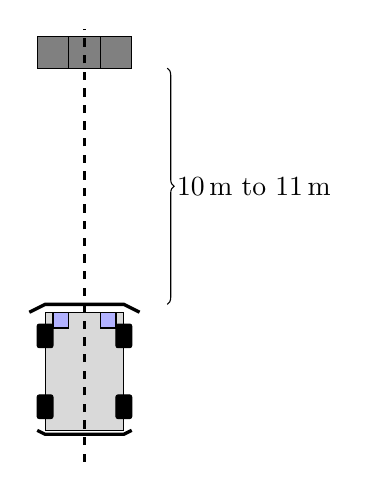
\begin{tikzpicture}
        \gokart{0}{0}{0}
    
        % Wall (three cubes)
        \draw[fill=gray] (-0.6,3) rectangle (-0.2,3.4);
        \draw[fill=gray] (-0.2,3) rectangle (0.2,3.4);
        \draw[fill=gray] (0.2,3) rectangle (0.6,3.4);
    
        % Dashed line from go-kart to wall (center axis)
        \draw[dashed, thick] (0,-2) -- (0,3.5);
    
        % Range brace annotation
        \draw [decorate, decoration = {brace, raise=10pt}] (0.7,3) -- (0.7, 0) node[pos=0.5,right=10pt,black]{\SIrange{10}{11}{\meter}};

        % Enlarged Radar sensor boxes
        \draw[fill=blue!30] (-0.4,-0.3) rectangle (-0.2,-0.1);

        \draw[fill=blue!30] (0.2,-0.3) rectangle (0.4,-0.1);
    \end{tikzpicture}
    \caption{Test scenario with dual front-mounted mmWave radar sensors.}
    \label{fig:test_scenario}
\end{figure}

The experimental setup is illustrated in Figure \ref{fig:test_scenario}, where two mmWave radar sensors are mounted at the front of a vehicle, providing overlapping fields of view to enhance environmental perception.
The dual-sensor configuration improves spatial coverage, reduces blind spots, and increases point density, resulting in more stable odometry processing compared to a single-sensor setup—an approach that aligns with multimodal methods for robust state estimation \cite{Multimodal_Offroad,HighSpeed_Estimation}.

By combining data from both sensors, including radial speed measurements derived from the Doppler effect, with the inertial measurement unit (IMU) for rotation compensation, the proposed system aims to ensure resilient odometry performance even under high-speed or degraded environmental conditions, where LiDAR-based odometry may fail \cite{HighSpeed_Estimation}.

Each radar perspective is processed independently and then merged into a single point cloud for further analysis.
This integration provides a more robust and reliable input to the odometry estimation pipeline, enabling the evaluation of radar-based odometry performance in realistic driving scenarios.

\subsection{Sub-Tasks}

The research objective, together with the constraints of using a dual-radar sensor, implied several practical sub-tasks:  
\begin{itemize}
    \item Designing a modular pipeline to acquire and decode synchronized radar data from both sensors.
    \item Investigating suitable sensor configurations to balance field of view, chirp bandwidth, update rate, and detection density.  
    \item Developing suitable mechanical mounts and selecting optimal sensor placement to ensure stability and maximize coverage.
    \item Applying RANSAC filtering on Doppler velocities to reject dynamic points and outliers.
    \item Implementing clustering methods to structure radar detections and isolate relevant features.  
    \item Optimizing the raw radar point cloud using additional information provided by the sensor itself (e.g., SNR, RCS, or range validity) to improve reliability before odometry processing.  
    \item Integrating Doppler velocity information into the odometry estimation process.   
    \item Employing submap aggregation to mitigate sparsity and improve stability. 
    \item Performing ICP alignment between submaps aggregated from both sensors to mitigate sparsity and noise. 
    \item Evaluating the influence of the dual-sensor arrangement on odometry accuracy and robustness. 
    \item Validating the complete system on real-world driving scenarios. 
\end{itemize}

As each sub-task builds upon the results of the previous one, the work followed an iterative and modular development approach, enabling gradual integration and continuous evaluation of the proposed system.  
The following sections detail the implementation and evaluation of each sub-task, culminating in a comprehensive radar-based odometry solution.
\section{IWR6843 Radar Interface and Configuration}
\label{sec:IWR6843 Radar Interface and Configuration}
The IWR6843AOPEVM development board from Texas Instruments features the IWR6843AOP, a high performance 4D mmWave FMCW sensor with Antenna On Package (AOP) design.
Although IWR6843AOP is intended for industrial applications and its complementary chip, AWR6843AOP, for automotive applications, IWR6843AOP was used in this project because it is available in the form of this development board and the two chips are identical in terms of their functionalities, only differing in compliance with automotive  industry \cite{iwr_awr_diff}.
Its small physical size, due to its AOP design, makes it an optimal choice for the desired mounting position, the go-kart's steering column.
\begin{figure}[!htbp]
    \centering
    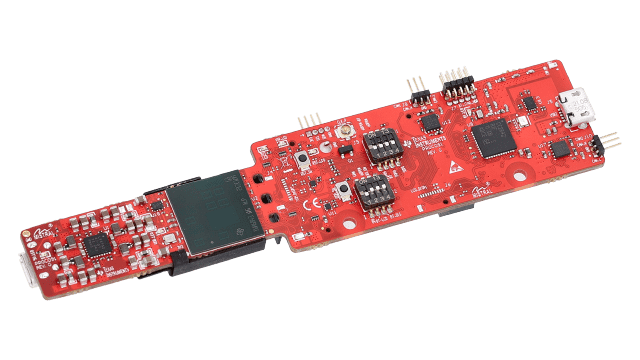
\includegraphics[width=0.7\linewidth]{images/iwr6843aopevm-angled.png}
    \caption{IWR6843AOP sensor\\
    \textit{Source: Texas Instruments, available at \url{https://www.ti.com/ds_dgm/images/fbd_swrs219f.gif}}}
    \label{fig:IWR6843AOP sensor}
\end{figure}
\par
The IWR6843AOP radar sensor operates within the frequency range of \SIrange{60}{64}{\giga\hertz} and integrates 4 receive (RX) and 3 transmit (TX) antennas, radio frequency (RF) front-end stages, analog signal processing, and digital signal processing (DSP).
It offers a wide range of communication interfaces including SPI, I2C, CAN-FD, UART and LVDS for raw data access and an Arm Cortex-R4F microcontroller for user-applications \cite{dev_board_page}.

\begin{figure}[!htbp]
    \centering
    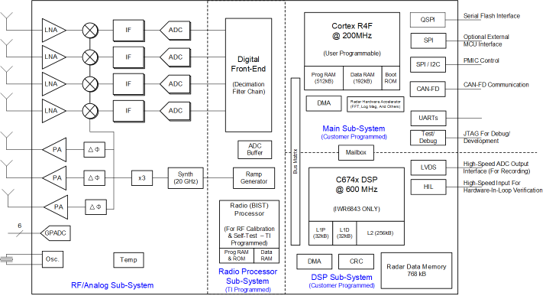
\includegraphics[width=1.0\linewidth]{images/blockdiagram.png}
    \caption{IWR6843AOP internal block diagram.\\
    \textit{Source: Texas Instruments, available at \url{https://www.ti.com/ds_dgm/images/fbd_swrs219f.gif}}}
    \label{fig:IWR6843AOP_internal}
\end{figure}

\FloatBarrier\noindent
Texas Instruments offers various demo applications for the development board that utilize the internal microcontroller for showcasing the radar sensor's capabilities in different specialized scenarios.
It was found out that most of them only use the radar sensor itself only for obtaining a point cloud, which points include spatial information in form of $x,y,z$ coordinates and a radial speed information (the prior mentioned four dimensions of the sensor).
Application-specific processing of the point cloud itself is executed on an external computation device.
\par
The main demo application ("mmWave SDK demo") allows a versatile customization of the radar sensor's operating parameters and its discrimination capabilities while outputting the point cloud via its UART interface, accessible via the on-board USB to UART converter.
Although the demo seems to be intended to be used only for demonstration purposes, many projects based on Texas Instruments' mmWave radar sensors utilize it, because it poses a generic solution for obtaining (close to) real-time point cloud data from the sensor without prior development of a custom user-application for the radar sensor's internal microcontroller.
This setup was therefore chosen for supplying the emergency braking system with data.

\subsection{Utilizing the mmWave SDK demo}
The "mmWave SDK demo" was developed by Texas Instruments for showcasing the abilities of their mmWave radar sensors.
It consists of the radar sensor itself, supplying close to real-time point cloud data and an online tool for visualization of the raw output data and for the creation of a sequence of commands used for configuration of the radar sensor's operating parameters and output \cite{mmwave_demo_doc}.
Due to the demo's simple structure and the radar sensor's generic output, the online application can be replaced by a custom application replicating the online tool's behavior for making use of the data.
\par
In the demo application, the radar sensor opens two UART connections.
One connection is bidirectional at a lower speed of \SI{115200}{\baud} which is used to configure the radar sensor by sending the previously mentioned sequence of commands. 
The second connection is unidirectional, from the radar sensor to the receiver, at a higher speed of \SI{921600}{\baud} and is used for outputting a constant data stream after the radar sensor received its configuration and a start command.
As the data packets are encoded in a proprietary format and therefore need to be parsed prior to further processing, a custom software module was written in C++ and later ported to Python.
The module handles the radar sensor's setup by sending a configuration file containing the sequence of initialization commands and the cyclic parsing of the encoded data packets.
The sequence of commands was generated with Texas Instruments' online tool, as it provided graphical feedback while making the necessary compromises involved in setting up the radar sensor's operating parameters.

\subsection{Sensor Data Output Format}
As the data packets, containing the individual frames, are encoded in a proprietary format, they need to be parsed to allow for further processing.
Each frame starts with a frame header and contains a number of TLVs (Type, Length, Value) in which the actual payload data is stored\cite{mmwave_demo_doc}.
\begin{figure}[!htbp]
    \centering
    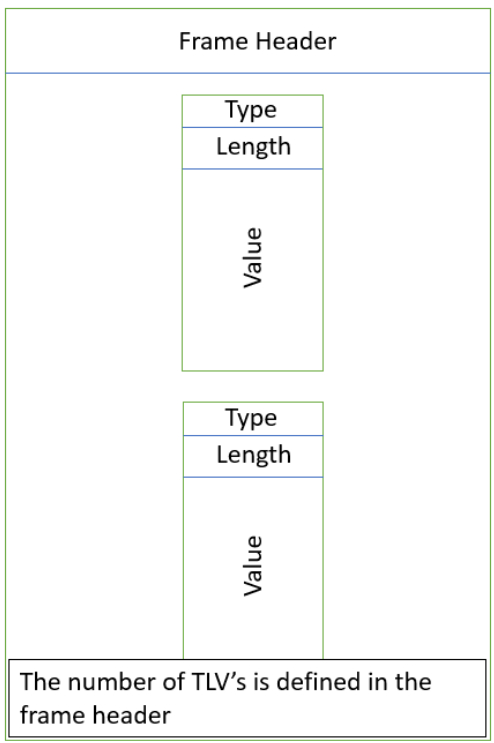
\includegraphics[width=0.4\linewidth]{images/UARTFrame.png}
    \caption{Frame structure. From \cite{mmwave_demo_output}.\\
    \textit{Source: Texas Instruments, available at \url{https://dev.ti.com/tirex/content/radar_toolbox_2_20_00_05/docs/software_guides/Understanding_UART_Data_Output_Format.html}}}
    \label{fig:UART data output format}
\end{figure}
\FloatBarrier\noindent
The frame's header has a total length of \SI{40}{\byte} and starts with a fixed magic word that denotes the start of each frame.
It also provides several other information in addition to the total packet length in bytes which is used to find the frame's end:
\begin{itemize}
    \item Magic Word: This value indicates the start of a new header, meaning that it can be used as a starting point for processing each frame.
    \item Total Packet Length: Total number of bytes in the frame (including the header) which can be used to calculate the frame's end.
    \item Platform: Indicates the device type and can be used for validating the radar sensor type. In the case of the device used for this project (IWR6843AOP) the expected value is "$0xA6843$".
    \item Number of TLVs: Total number of TLV's that exist in that specific frame.
\end{itemize}
\begin{figure}[!htbp]
    \centering
    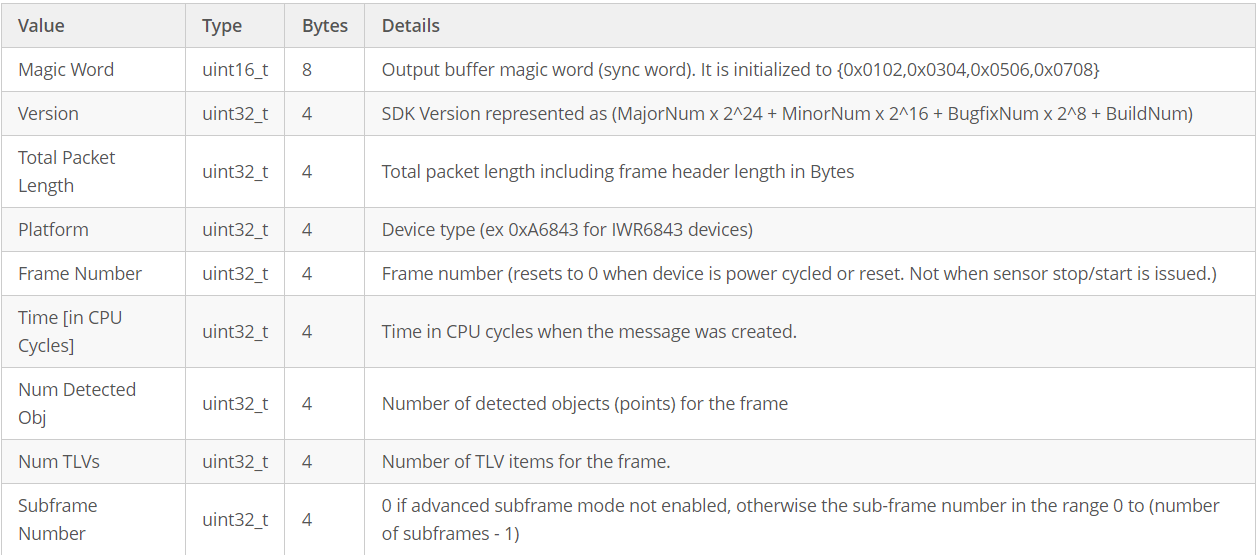
\includegraphics[width=1.0\linewidth]{images/FrameFormatHeader.png}
    \caption{Frame header format. From \cite{mmwave_demo_output}.\\
    \textit{Source: Texas Instruments, available at \url{https://dev.ti.com/tirex/content/radar_toolbox_2_20_00_05/docs/software_guides/Understanding_UART_Data_Output_Format.html}}}
    \label{fig:Frame header format}
\end{figure}
\FloatBarrier\noindent
The frame contains one or more TLVs after its header.
Each TLV has a header itself in which it specifies its length and which type of data (point cloud, doppler heatmaps, statistics, ...) is contained inside.
Each TLV type needs to be decoded differently, as it represents a different type of data.
\begin{figure}[!htbp]
    \centering
    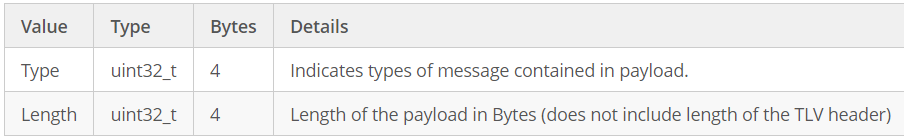
\includegraphics[width=0.95\linewidth]{images/TLVHeader.png}
    \caption{TLV header format. From \cite{mmwave_demo_output}.\\
    \textit{Source: Texas Instruments, available at \url{https://dev.ti.com/tirex/content/radar_toolbox_2_20_00_05/docs/software_guides/Understanding_UART_Data_Output_Format.html}}}
    \label{fig:TLV header format}
\end{figure}
\FloatBarrier

\subsection{Sensor-Tuning}
As some operating parameters influence each other, their selection must be done carefully while observing the influence of the trade-offs involved.
This could be referred to as "sensor tuning" and is a critical step because it directly impacts the system's accuracy and performance.

The following operating parameters can be tuned:
\begin{itemize}
    \item Frame rate
    \item Range resolution
    \item Maximum unambigious range
    \item Maximum radial velocity
    \item Radial velocity resolution
\end{itemize}

Tuning these operating parameters introduces trade-offs by influencing each other in the following ways:
\begin{table}[h]
    \centering
    \resizebox{\columnwidth}{!}{
    \begin{tabular}{|l|l|p{3.5cm}|p{3.5cm}|p{3.5cm}|}
        \hline
        \textbf{Tuning Parameter} & \textbf{Effect on Performance} & \textbf{Related HW Block} & \textbf{Trade-Off} \\
        \hline
        Frame Rate & Higher FPS = faster updates but more processing load & C674x DSP, Radar Data Memory & Higher FPS reduces maximum range \\
        \hline
        Range Resolution & Higher resolution = better object separation & ADC, 1D FFT (Range FFT) & Higher resolution reduces max range \\
        \hline
        Maximum Range & Determines farthest detectable object & RF Front-End, PA, LNA, ADC & Higher range lowers resolution \\
        \hline
        Radial Velocity Resolution & Improves speed accuracy & DSP, 2D FFT (Doppler FFT) & Higher resolution requires more chirps \\
        \hline
        Maximum Radial Velocity & Detects fast-moving objects & Chirp rate, TX Antennas, 2D FFT & Higher max velocity reduces resolution \\
        \hline
    \end{tabular}
    }
    \caption{Radar System Tuning Parameters and Trade-offs}
    \label{tab:mmWave_Sensor_Parameters}
\end{table}
The resulting overall accuracy of the velocity and distance measurements is again dependent on these operating parameters:
\begin{itemize}
\item \textbf{Radial velocity accuracy:} A fine balance between velocity resolution and frame rate must be maintained to ensure precise Doppler shift measurements. Lower resolution results in rounded velocity values, while an excessively high frame rate may introduce computational bottlenecks.
\item \textbf{Distance accuracy:} Optimizing range resolution and maximum range ensures that detected objects are positioned accurately within the environment. Increasing range often sacrifices resolution, leading to potential inaccuracies in close-range detections.
\item \textbf{Signal processing considerations:} The FFT calculation parameters directly affect both range and Doppler calculations, influencing the ability to distinguish between objects and detect small velocity variations.
\end{itemize}

This shows that finding exact values for the operation parameters by adjusting them while carefully watching their influences is crucial and heavily dependent on the particular application.
The test scenario required a frame rate of approximately 30Hz to balance responsiveness and computational load, together with sufficient range and velocity coverage to capture typical vehicle dynamics.

The resulting configuration yielded the following operating parameters:
\begin{itemize}
\item Frame rate: \SI{30}{\frame\per\second}
\item Range resolution: \SI{0.047}{\meter}
\item Maximum unambiguous range: \SI{9.78}{\meter}
\item Maximum radial velocity: \SI{8.01}{\meter\per\second}
\item Radial velocity resolution: \SI{0.51}{\meter\per\second}
\end{itemize}

Tuning and choosing the sensor's parameters carefully is extremely important as it defines the accuracy of 
therefore influences the reliability of the entire radar system.
Fine-tuning these settings ensures that the sensor operates optimally, enabling more precise self-speed estimation and overall system performance.
The accuracy of radial speed estimation and distance measurements depends directly on the tuning of these parameters. A poorly configured sensor can result in erroneous velocity estimations, unreliable object detection, or excessive noise in Doppler measurements. 
An example of the influence of the selection of the correct parameters on the output point cloud of the radar sensor can be found in Fig.~\ref{fig:IWR6843AOP Calibration example2 for the sensor}.

\begin{figure}[!htbp]
    \centering
    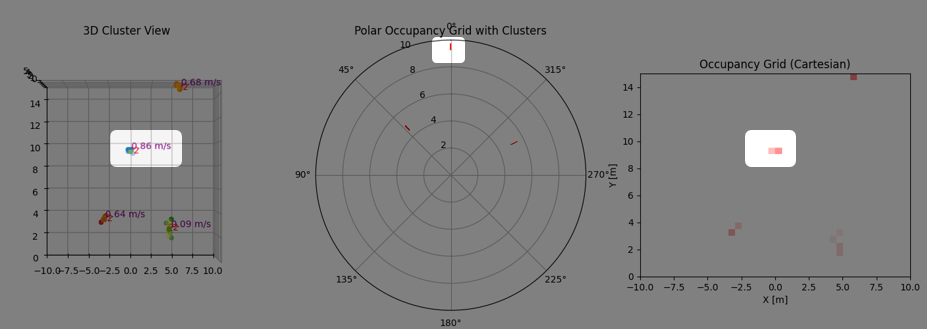
\includegraphics[width=1.0\linewidth]{images/calib_ex.png}
    \caption{Output of the IWR6843AOP prior sensor tuning.}
    \label{fig:IWR6843AOP Calibration example for the sensor}
\end{figure}

\begin{figure}[!htbp]
    \centering
    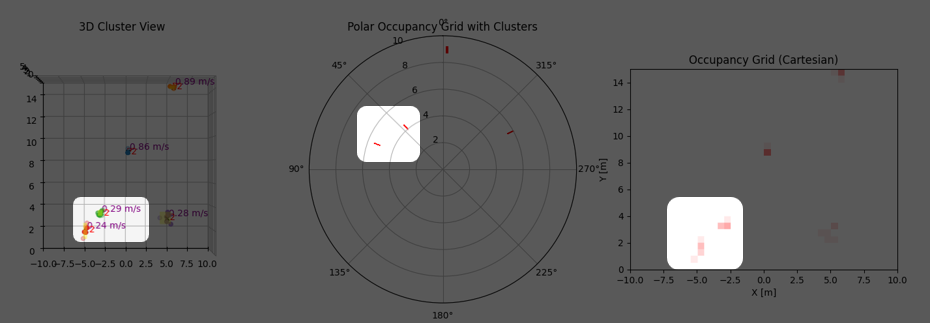
\includegraphics[width=1.0\linewidth]{images/calib_ex2.png}
    \caption{Output of the IWR6843AOP after sensor tuning.}
    \label{fig:IWR6843AOP Calibration example2 for the sensor}
\end{figure}

\subsection{Dual Sensor-Tuning} 
In addition to the individual calibration of each radar, further adjustments were required to enable a dual-sensor configuration with overlapping fields of view. 
The sensors were physically rotated around the $Z$-axis to widen the horizontal coverage and tilted by $15^\circ$ around the $X$-axis to prevent ground reflections and reduce clutter in the point clouds. 

\subsubsection{Chirp Calibration with Frequency Shift} 
Although both sensors operated under the same high-level parameters, their chirps had to be tuned to avoid mutual interference and ghost detections. 
To achieve this, each radar was configured to occupy only 2\,GHz of the available 4\,GHz bandwidth, introducing a frequency shift between the sensors. 
The resulting chirp design was derived using the Texas Instruments \textit{mmWave Sensing Estimator} tool \cite{understanding_uart}, which provides interactive validation of scene-dependent parameters, chirp design, and power consumption estimates. 
This configuration allowed the sensors to operate simultaneously without cross-talk while maintaining sufficient range resolution and velocity accuracy. 

\subsubsection{Geometric Transformations} 
To merge both radar outputs into a consistent reference frame, rigid-body transformations were applied to compensate for rotation, tilt, and translation offsets between the sensors. 
Each radar detections were first processed in its local coordinate frame and then transformed into the vehicle-centric frame before fusion into a single point cloud. 

Figures~\ref{fig:dualSensorCalib_rawComparison}--\ref{fig:dualSensorCalib_RANSACComparison} illustrate the effect of this calibration process at different processing stages: 
\begin{itemize} 
    \item \textbf{Raw point clouds:} Before calibration (Fig.~\ref{fig:dualSensorCalib_rawComparison}a), the detections from each sensor appear misaligned, producing duplicated landmarks. After applying the transformations (Fig.~\ref{fig:dualSensorCalib_rawComparison}b), both perspectives are fused into a coherent scene. 
    \item \textbf{Clustered view:} When clustering is applied, the uncalibrated data (Fig.~\ref{fig:dualSensorCalib_clusterComparison}a) shows inconsistent cluster centers, while the calibrated version (Fig.~\ref{fig:dualSensorCalib_clusterComparison}b) produces compact and aligned clusters. 
    \item \textbf{RANSAC Doppler fitting:} Similarly, Doppler–azimuth consistency improves after calibration. Uncalibrated detections (Fig.~\ref{fig:dualSensorCalib_RANSACComparison}a) yield noisier distributions, while the calibrated outputs (Fig.~\ref{fig:dualSensorCalib_RANSACComparison}b) produce smoother fits with fewer outliers. 
\end{itemize} 

The transformed data thus provides a coherent and stable input for the odometry estimation pipeline, ensuring that static landmarks are consistently aligned across both sensors.  

\begin{figure}[ht]
    \centering
    \begin{subfigure}[b]{0.45\textwidth}
        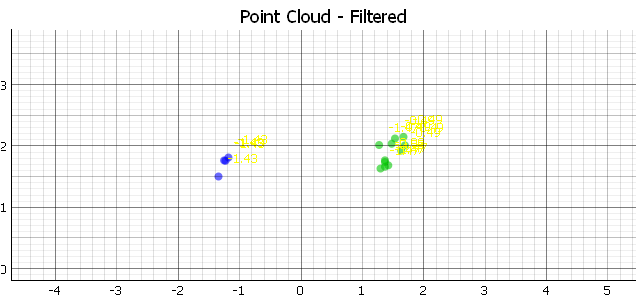
\includegraphics[width=\textwidth]{images/dualSensorCalib_2mts.png}
        \caption{Raw point cloud before calibration}
    \end{subfigure}
    \hfill
    \begin{subfigure}[b]{0.45\textwidth}
        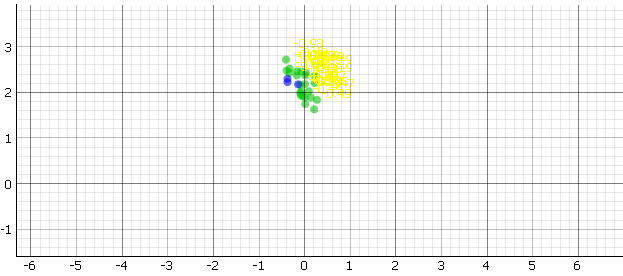
\includegraphics[width=\textwidth]{images/AFTERdualSensorCalib_2mts.png}
        \caption{Raw point cloud after calibration}
    \end{subfigure}
    \caption{Dual-sensor raw detections before and after applying geometric transformations.}
    \label{fig:dualSensorCalib_rawComparison}
\end{figure}

\begin{figure}[ht]
    \centering
    \begin{subfigure}[b]{0.3\textwidth}
        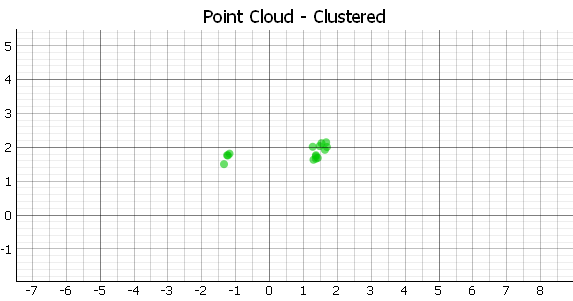
\includegraphics[width=\textwidth]{images/dualSensorCalibCluster_2mts.png}
        \caption{Clustered detections before calibration}
    \end{subfigure}
    \hfill
    \begin{subfigure}[b]{0.3\textwidth}
        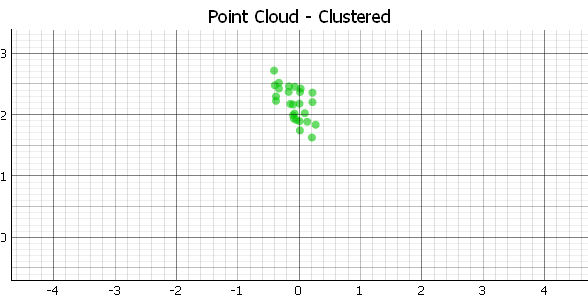
\includegraphics[width=\textwidth]{images/AFTERdualSensorCalibCluster_2mts.png}
        \caption{Clustered detections after calibration}
    \end{subfigure}
    \caption{Effect of calibration on cluster alignment across sensors.}
    \label{fig:dualSensorCalib_clusterComparison}
\end{figure}

\begin{figure}[ht]
    \centering
    \begin{subfigure}[b]{0.3\textwidth}
        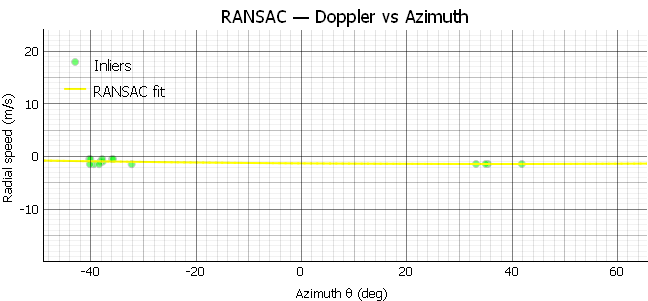
\includegraphics[width=\textwidth]{images/dualSensorCalibRANSAC_2mts.png}
        \caption{RANSAC Doppler fitting before calibration}
    \end{subfigure}
    \hfill
    \begin{subfigure}[b]{0.3\textwidth}
        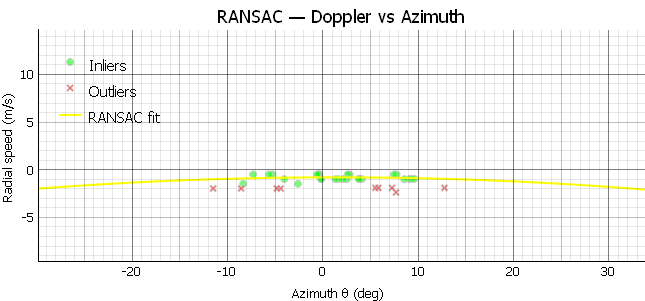
\includegraphics[width=\textwidth]{images/AFTERdualSensorCalibRANSAC_2mts.png}
        \caption{RANSAC Doppler fitting after calibration}
    \end{subfigure}
    \caption{Improvement in Doppler-azimuth consistency after calibration.}
    \label{fig:dualSensorCalib_RANSACComparison}
\end{figure}

\FloatBarrier
%% \section{Theoretical Foundations: Mathematical Models and Algorithms for Radar-Based Object Detection}
%% \label{sec:Mathematical Models and Algorithms for Radar-Based Object Detection}

\section{Pipeline implementation: Modules implemented and mathematical explanation}
\label{sec:Mathematical Models and Algorithms for Radar-Based Object Detection}
As the radar sensor outputs its raw data in frames which contain a raw point cloud, a modular processing pipeline was developed.
This pipeline consists of different modules implementing the needed stages for pre-processing the sensor's data, filtering the point cloud, clustering and object detection.
The modular design allows the modification and adaption to different environments.
\par
In a pre-processing stage, the sensor's raw data frames, obtained via UART, are decoded and translated into frames containing individual points in a usable format with information about their $x,y,z,v_{r}$ and $SNR$ values.
They are then passed into a "Frame Aggregator" which stores a certain amount of frames in order to supply the later stages with the data from multiple frames and thus compensate for possible data sparsity.
The aggregated data is filtered by multiple filtering stages, starting with static parameters for the spatial dimension and the SNR, followed by a dynamic filtering stage using a comparison of the vehicle's estimated self-speed to the points' speeds for filtering.
The filtered points are then clustered using a two-stage approach and forwarded to the brake controller for object detection. The reason for the 2 stages of clustering is that for any given object that may be detected there would be noise or segmentation caused by some space between objects. So this 2 stages help us discard information that could be just a reflection and focus into the points that are considered as objects. This being done by having a permissive first stage, and afterwards a strict clustering stage to be able to label an object with a cluster ID for further processing.
\begin{figure}[!htbp]
    \centering
    \resizebox{0.48\textwidth}{!}{
        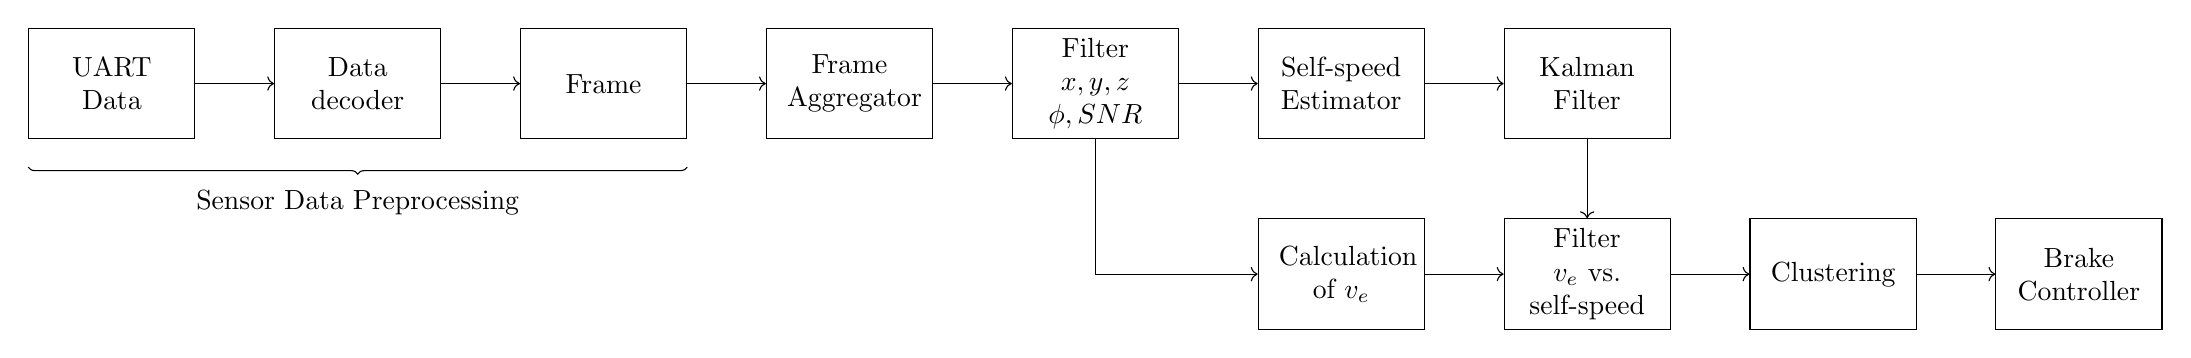
\begin{tikzpicture}
            % Block styles
            \tikzstyle{block} = [rectangle, draw, text width=4.5em, text centered, minimum width=6em, minimum height=4em]
            \tikzstyle{block_dashed} = [rectangle, draw, text width=2em, text centered, minimum width=4em, minimum height=4em, dashed]
            % Input and output
            \node[block] (uart) {UART\\Data};
            \node[block, right=of uart] (decoder) {Data decoder};
            \node[block, right=of decoder] (frames) {Frame};
            \node[block, right=of frames] (frame_aggr) {Frame\\Aggregator};
            \node[block, right=of frame_aggr] (coord_filter) {Filter\\$x,y,z$\\$\phi,SNR$};
            \node[block, right=of coord_filter] (self_speed_estim) {Self-speed Estimator};
            \node[block, right=of self_speed_estim] (self_speed_kalman) {Kalman Filter};
            \node[block, below=of self_speed_estim] (ve_speed_calc) {Calculation\\of $v_{e}$};
            \node[block, right=of ve_speed_calc] (ve_filter) {Filter\\$v_{e}$ vs. self-speed};
            \node[block, right=of ve_filter] (clustering) {Clustering};
            \node[block, right=of clustering] (brake_controller) {Brake\\Controller};
            % Connections
            \draw[->] (uart) -- (decoder);
            \draw[->] (decoder) -- (frames);
            \draw[->] (frames) -- (frame_aggr); % Connection from antenna to RF amplifier
            \draw[->] (frame_aggr) -- (coord_filter);
            \draw[->] (coord_filter) -- (self_speed_estim);
            \draw[->] (coord_filter.south) |- (ve_speed_calc.west);
            \draw[->] (self_speed_estim) -- (self_speed_kalman);
            \draw[->] (self_speed_kalman) -- (ve_filter);
            \draw[->] (ve_speed_calc) -- (ve_filter);
            \draw[->] (ve_filter) -- (clustering);
            \draw[->] (clustering) -- (brake_controller);

            \draw [decorate, decoration = {brace, mirror, raise=10pt}] (uart.south west) --  (frames.south east) node[pos=0.5,below=15pt,black]{Sensor Data Preprocessing};
        \end{tikzpicture}
    }
    \caption{Block diagram of the pipeline}
    \label{fig:block_diag_pipeline}
\end{figure}

\FloatBarrier\noindent

%\begin{figure}[!htbp]
%    \centering
%    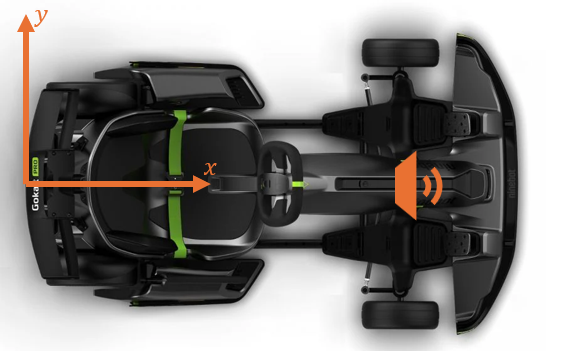
\includegraphics[width=1.0\linewidth]{images/ninebot.png}
%    \caption{Schematic sensor distribution}
%    \label{fig: One sensor is located in the front of the test vehicle}
%\end{figure}
%\FloatBarrier\noindent

\subsection{Frame Aggregator}
\label{sec:Frame Aggregator}
The decoded frames are passed into a frame aggregator stage as a first step, which utilizes data aggregation to reduce possible data sparsity of individual frames. 
Data aggregation involves combining multiple consecutive data sets to create a more comprehensive and reliable dataset for processing. This approach increases both useful information and noise, but ultimately enhances the quality of radar point clouds for object detection and tracking stability.
For point clouds from radar sensors, aggregating multiple frames enhances data consistency and density, improving the system’s ability to reconstruct objects and detect motion patterns.

\subsubsection{Single Frame}
Using radar point cloud data from a single frame has inherent limitations, which can lead to incomplete or misleading detections:
\begin{itemize}
    \item A single frame may not capture enough points, leading to failed detections or incomplete object reconstruction.
    \item Limited point data can cause objects to appear fragmented or indistinguishable from noise.
\end{itemize}

\begin{figure}[!htbp]
    \centering
    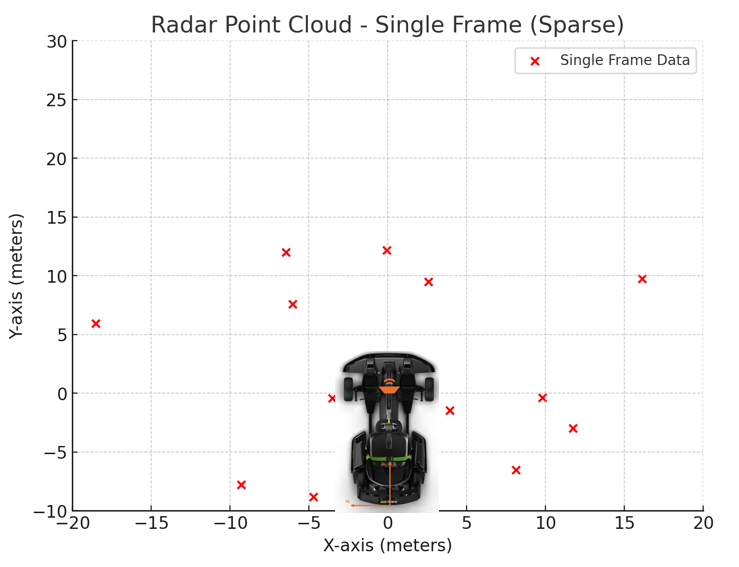
\includegraphics[width=0.5\linewidth]{images/singleframe.png}
    \caption{Single Frame visualization.}
    \label{fig: Single Frame visualization}
\end{figure}

Consequently, it is difficult to precisely rebuild or map complex objects due to the limited points in the point cloud and information contained in a single radar frame, which results in ambiguity and uneven detection performance.
This ambiguity can result in the erroneous detection of a large object or the merging of two different objects into one, as the clustering or detection algorithm may malfunction, not due to inherent flaws in the algorithm itself, but rather due to the inherent flaws in the data. This phenomenon occurs when two or more objects are in close proximity from each other, but can not be distinguished from each other because of the lack of points in a single frame.

To mitigate these issues, frame aggregation can be leveraged, an approach supported by the Law of Large Numbers (LLN). By accumulating multiple frames, the impact of random variations can be reduced, such as:
\begin{equation}
    \frac{\sigma^2}{N}
    \label{eq:variance_per_sample_size}
\end{equation}
This leads to a more statistically stable representation of objects; which means that the larger the sample is, the less effect the noise will have. Additionally, variance reduction helps to filter out erroneous detections while improving the reliability of motion estimation.

\subsubsection{Multiple Frames}
In contrast, the aggregation of multiple frames can significantly enhance object detection capabilities.
Using this technique the algorithm can be tricked, by making it believe that there is more information that it was actually obtained from the single frame. This comes with the drawback that there will be some older data inside the processed frame.
\begin{figure}[!htbp]
    \centering
    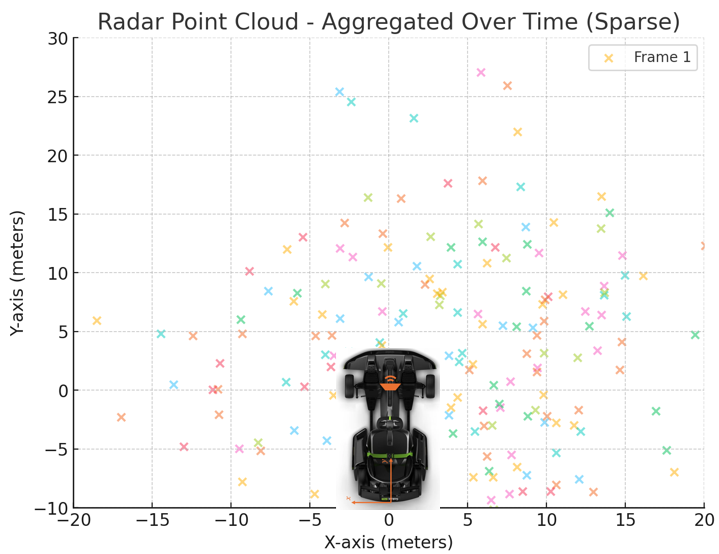
\includegraphics[width=0.5\linewidth]{images/multiframe.png}
    \caption{Frame Aggregation visualization.}
    \label{fig: Frame Aggregation visualization}
\end{figure}

This aggregation approach improves the accuracy of velocity and trajectory estimations, strengthens object identification's resilience against transient noise, and reduces problems related to sparse data.
It was implemented by using a stack with a fixed size, executing a "pop" operation prior to the insertion of the new frame at the stack's end.
The point cloud containing the points of all frames stored in the frame aggregator is then passed to the next stage.
\subsection{"$x,y,z,\phi,SNR$" Filter}
The point cloud's points are passed through a first static filtering stage to remove points caused by noise, clutter or targets outside of the area of interest before being used for further processing.
This static filtering stage consists of four different filters, filtering out points by different attributes:
\begin{enumerate}
    \item Filtering by $SNR$: All points with a $SNR$ lower than \SI{12}{\deci\bel} are filtered out to remove points with a low signal and those that might be caused by noise or clutter.
    \item Filtering by $z$ coordinate: All points below a $z$ value of \SI{0}{\meter} and above \SI{2}{\meter} are filtered out to remove points caused by the ground or the ceiling.
    \item Filtering by $y$ coordinate: All points below a $y$ value of \SI{0.3}{\meter} are filtered out to remove points created by the driver's feet.
    \item Filtering by $\phi$: All points with an azimuth bigger than \SI{85}{\degree} are filtered out to remove points that are outside the area of interest.
\end{enumerate}
\textit{Note: The origin of the points' coordinate system is the sensor itself, so a coordinate of $(\SI{0}{\meter},\SI{0}{\meter},\SI{0}{\meter})$ is essentially at the sensor's mounting position and therefore approx. \SI{0.3}{\meter} above the ground.}
\par
As the static filtering stage only keeps points which are relevant in terms of there spatial position and $SNR$ for the following stages, it effectively decreases the computation time of each frame and prevents the following stages from processing invalid data.
The filtered point cloud is then passed to the next stages, the self-speed estimator and the dynamic filtering stage.

\begin{figure}[!htbp]
\centering
\begin{subfigure}{0.24\textwidth}
  \centering
  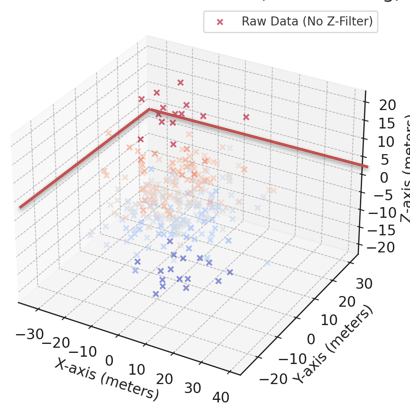
\includegraphics[width=\textwidth]{images/No_filter.png}
  \caption{Input}
\end{subfigure}
\begin{subfigure}{0.24\textwidth}
  \centering
  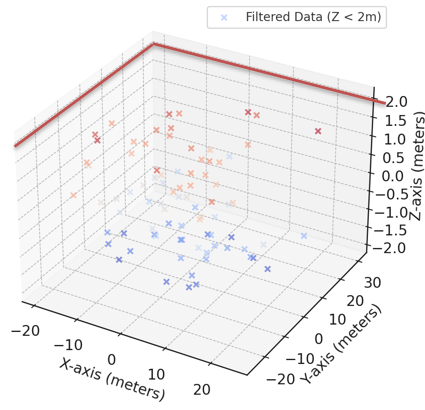
\includegraphics[width=\textwidth]{images/filter.png}
  \caption{Output}
\end{subfigure}
\caption{Example visualization of the input and output when filtering by the value of the $z$ coordinate.}
\label{fig:static_filter_z_example}
\end{figure}
\FloatBarrier\noindent

%% [20/03/2025] Leander: Rework done, commentend out bc. probably not needed anymore
%% ---------------------------------------
\begin{comment}
(effectively the radar sensor's mounting height as the coordinate's origin is at the sensor; approx. \SI{30}{\centi\meter} above ground) and \SI{2}{} 
Physical filtering further refines the data, this by removing points that can be considered as environmental noise or clutter, points outside the sensor’s effective monitoring area, or points whose radar cross-section (RCS) values fall below a predetermined threshold.
By mentioning the sensor effective monitoring area it is considered as area that the sensor will gather the information, process it and then give it as a result. But we might not be interested in all of this information.

\begin{figure}[!htbp]
\centering
\begin{subfigure}{0.24\textwidth}
  \centering
  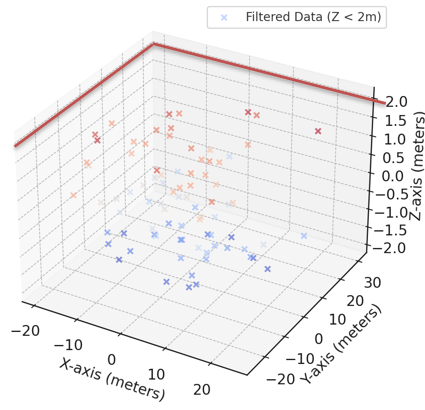
\includegraphics[width=\textwidth]{images/filter.png}
\end{subfigure}
\begin{subfigure}{0.24\textwidth}
  \centering
  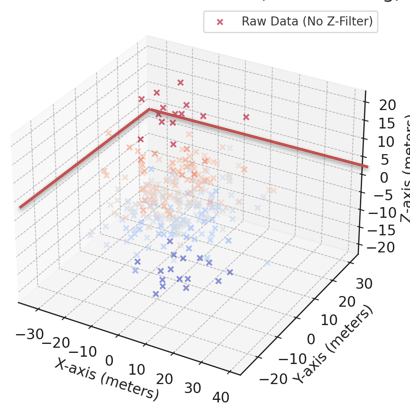
\includegraphics[width=\textwidth]{images/No_filter.png}
\end{subfigure}
\caption{The physical filters help us consider only information that may be caught by the sensor, but is of no use for us.}
\label{fig:remote_controller_components}
\end{figure}

For the project application and sensor location, it is considered that a Z-axis filter it is needed. As it will add more points that we will process if we don't discard them for the processing of the point-cloud.

This same concept may apply for other physical values of the point-cloud data, this being radial speed. If a point with a radial speed that is considered just ridiculous, then we add that point to the discarded data.
\end{comment}
\subsection{Self-speed Estimator}
\label{sec:self-speed_estimator}
The vehicle's self-speed is used for distinguishing between points of stationary and moving objects and filtering out the points of moving objects in a later block of the pipeline.
It therefore needs to be determined in a reliable way.
Traditional approaches usually utilize external sensors such as wheel encoders, Global Positioning System (GPS), or Inertia Measurement Units (IMUs).
In this project, a technique was developed that determines the vehicle's self-speed only by processing the point cloud's data.
An angle $\phi_{p}$ was defined between each individual point of the point cloud and the radar sensor's centerline:
\par
\begin{figure}[!htbp]
    \centering
    %\resizebox{0.48\textwidth}{!}{
        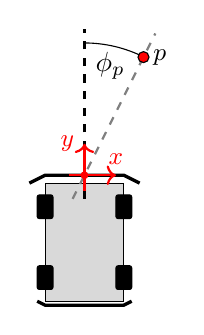
\begin{tikzpicture}
            \gokart{0}{0}{0}

            \coordinate(O) at (0,0);
            \coordinate(P) at (0.75,1.5);
            \coordinate(A) at (0,1.5);

            \draw[dashed, thick, gray] ($(P)!1.2!(O)$) -- ($(O)!1.2!(P)$);
            \draw[dashed, thick] ($(A)!1.2!(O)$) -- ($(O)!1.24!(A)$);
            \draw pic["$\phi_{p}$", draw=black, angle radius=1.68cm, angle eccentricity=0.85] {angle=P--O--A};
            \draw[fill=red] (P) circle (0.07) node [right] {\small $p$};

            \draw[->, thick, red] (-0.2,0) -- (0.4,0) node[above] {\small $x$};
            \draw[->, thick, red] (0,-0.2) -- (0,0.4) node[left] {\small $y$};
            \fill[red] (0,0) circle (0.05);
        \end{tikzpicture}
    %}
    \caption{Definition of the angle $\phi_{p}$}
    \label{fig:def_angle_phi}
\end{figure}
\FloatBarrier\noindent
These angles $\phi_{p}$ can be calculated using the points' cartesian position information:
\begin{equation*}
    \phi_{p} = arctan\left(\frac{x_{p}}{y_{p}}\right)
    \label{eq:calc_angle_phi}
\end{equation*}
A curve $v(\phi)$ is fitted through the points with their angles $\phi_{p}$ serving as the independent variable and their radial speeds $v_{r,p}$ as the dependent variable.
The curve's value $v(\phi = \SI{0}{\degree})$ then gives an estimation for the vehicle's self speed.
\par
This is possible because the perceived radial speed $v_{r,p}$ of a point related to a stationary target is dependent on the angle $\phi_{p}$ and follows a cosine when being passed at a certain speed $v_{0}$:
\begin{equation*}
    v_{r,p}(v_{0},\phi_{p}) = -v_{0} \cdot cos(\phi_{p})
\end{equation*}
At $\phi = \SI{0}{\degree}$, the radial speed is therefore equal to the vehicle's self speed.
Because there is rarely a point exactly at \SI{0}{\degree} and the radial speeds of the points also include noise, the approach uses all available points after the first filtering stage to fit a curve and effectively give the best possible estimation.
The implementation uses a least squares polynomial regression approach to fit a 2nd order polynomial (see \cite{numpy_polyfit}), which is sufficient in this case as the angle $\phi$ is defined in a way that $\phi_{p} = \left[-\frac{\pi}{2},\frac{\pi}{2}\right]$, so the cosine can be approximated by a 2nd order polynomial:
\begin{equation*}
    cos(\phi_{p}) \approx a \cdot \phi_{p}^2 + b \quad with\enspace \phi_{p} = \left[-\frac{\pi}{2},\frac{\pi}{2}\right]
\end{equation*}
Multiple runs of this algorithm with recorded test data proved the technique's principle.
\begin{figure}[!htbp]
    \centering
    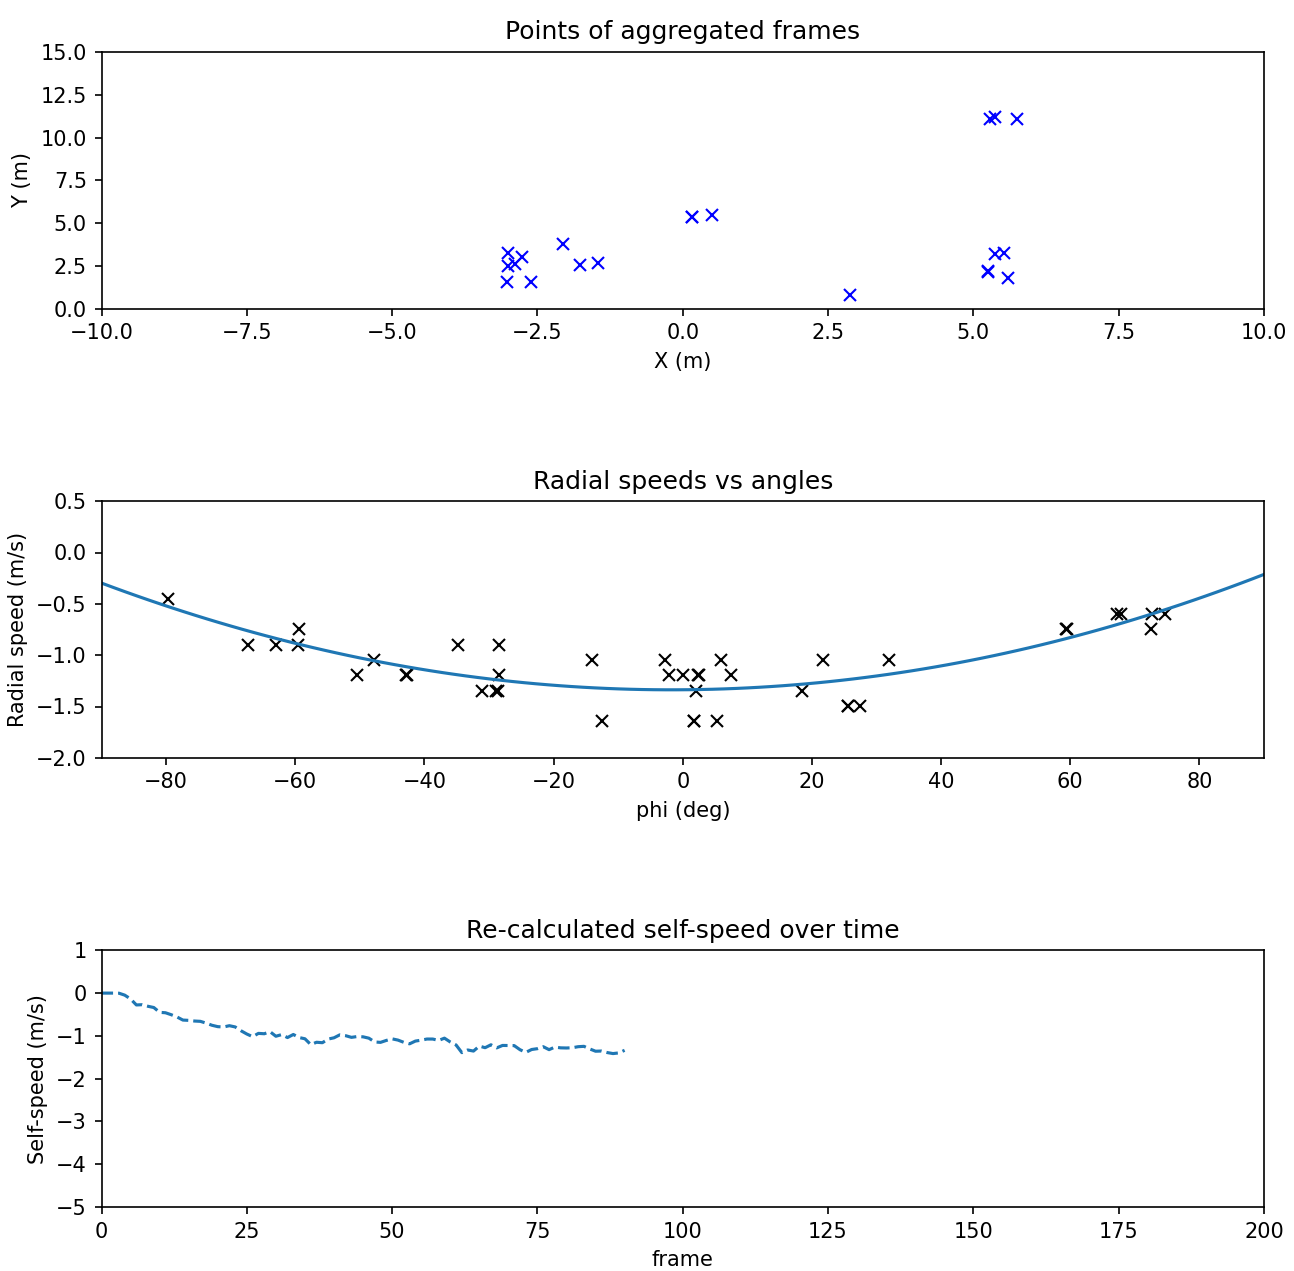
\includegraphics[width=1.0\linewidth]{images/self_speed_reality.png}
    \caption{Test run with recorded data and visualization.}
    \label{fig:self_speed_test_data}
\end{figure}
\FloatBarrier\noindent
During tests, the self-speed estimated by this technique matched the go-kart's built-in speed indicator with some small static offset but also showed heavy fluctuations from time to time when the radar sensor's output only contained a small amount of points.
Although this influence could be reduced by tuning the amount of frames stored in the frame aggregator, a stage containing a Kalman Filter was added after the self-speed estimation before the self-speed value is passed to the following pipeline blocks.



%% [20/03/2025] Leander: Rework done, commentend out bc. probably not needed anymore
%% ---------------------------------------
\begin{comment}

\todo {This whole chapter needs to be done again}
The estimation of a vehicle’s self-speed is a fundamental requirement for autonomous navigation and advanced driver-assistance systems (ADAS). Traditional methods often rely on external sensors such as wheel encoders, GPS, or IMUs to determine vehicle velocity. However, in this project, no external sensor was used for speed estimation. Instead, velocity was estimated exclusively using data from an mmWave radar sensor, leveraging its Doppler measurements to infer motion.

The proposed approach estimates ego-motion (velocity) of the vehicle by analyzing the radial velocity obtained from the radar point cloud. The mmWave radar measures the Doppler shift of each detected point, which corresponds to the relative velocity of objects with respect to the sensor. Assuming that all detected objects are static, the observed Doppler velocities can be directly attributed to the vehicle’s own motion.

\begin{figure}[!htbp]
    \centering
    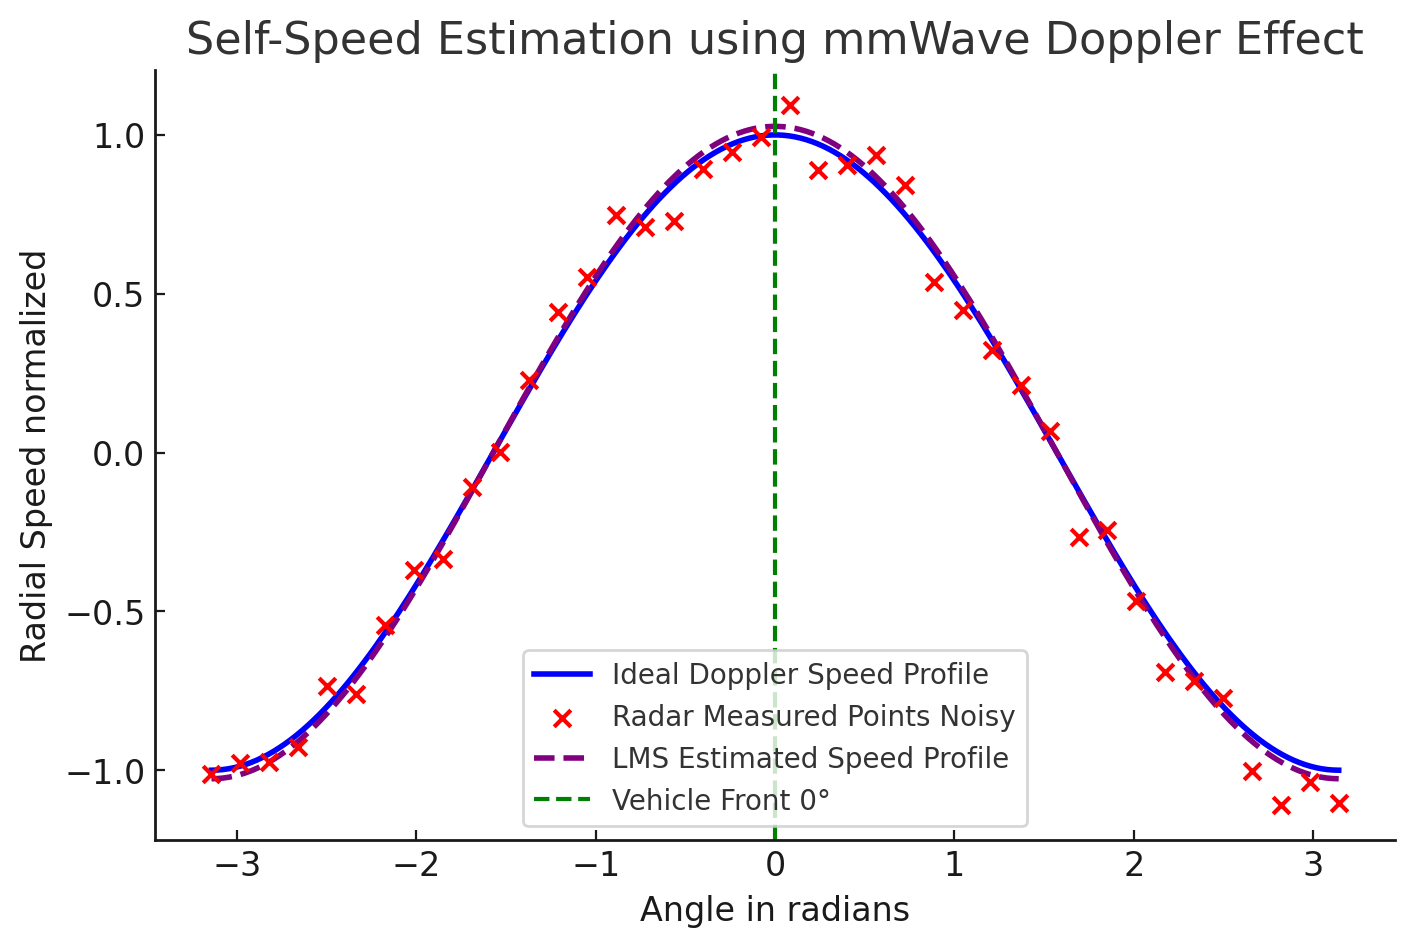
\includegraphics[width=1.0\linewidth]{images/Self_Speed_Doppler.png}
    \caption{Self-Speed Estimation Using MmWave Doppler Effect}
    \label{fig: Self-Speed Estimation Using MmWave Doppler Effect}
\end{figure}
\FloatBarrier\noindent
To estimate speed accurately, radial velocities are fitted to a cosine function that simulates the Doppler shift as a function of detecting angle.  The estimation must be improved, nevertheless, by using an adaptive filtering technique because of measurement noise and differences in detected sites.  The speed estimate is iteratively adjusted in this study by minimizing the error between the measured velocities and the expected cosine profile using the Least Mean Squares (LMS) technique.  This makes it possible to estimate self-speed accurately and reliably without the need for further external sensors.

\subsubsection{Doppler Effect and Speed estimation}

The Doppler effect is a fundamental principle in radar-based velocity estimation. When a vehicle moves, the mmWave sensor measures the radial velocity of detected objects based on the frequency shift of the reflected radar waves. This Doppler shift can be expressed as:

-------------------------------

Estimating the ego-motion (velocity) of a vehicle using radar point clouds can be achieved by analyzing the measured radial velocities (Doppler Shift) from radar returns and solving a least-squares optimization problem. The radar sensor provides radial velocities, which are essentially the component of the actual velocity vector along the radar's line of sight.
However this velocity will shift depending on the angle that it was obtained. For example the most precise velocity is the one that comes from the objects in front of the vehicle, but the ones in the side will have a certain 'error'.

For obtaining this estimations we need:
\begin{itemize}
    \item Input preparation: Each radar detection provides two primary measurements:
    \begin{itemize}
        \item Angle to the target.
        \item Radial speed (Doppler velocity).
    \end{itemize}
    \item Forming the Data Structure: Each radar point is processed individually, computing the angle  (in radians or degrees) and associating it with the measured radial speed. 
    \item Polynomial Regression (Least Squares Fit): To estimate the ego-velocity, the method fits a polynomial (typically first-order for simplicity) to the radial velocities as a function of the angles. 

    \[
    \min_{a,b} \sum_{i} \left( v_{\text{radial}, i} - (a \phi_i + b) \right)^2
    \]


    \item Velocity Estimation: After obtaining coefficients from the polynomial fit, the ego-velocity estimate is derived from evaluating the polynomial at the central angle:
    \FloatBarrier\noindent
    \begin{equation}
        V_{\text{ego}} = b
        \label{eq:velocity_ego_vehicle}
    \end{equation}
    
\end{itemize}

\end{comment}
\subsection{Kalman Filter}
The Kalman filter is a widely used mathematical algorithm to improve the accuracy of measurements by reducing the noise and uncertainty inherent in sensor data. This is done via estimations of what could be the next state using prior measurements to obtain this "next" state. 
To enhance the accuracy of the self-speed estimation, a 1D Kalman (meaning that it is used to estimate only one state) filter was implemented.
This filter estimates the vehicle's exact velocity based on the provided radar-based seld speed estimation data.
\begin{figure}[!htbp]
    \centering
    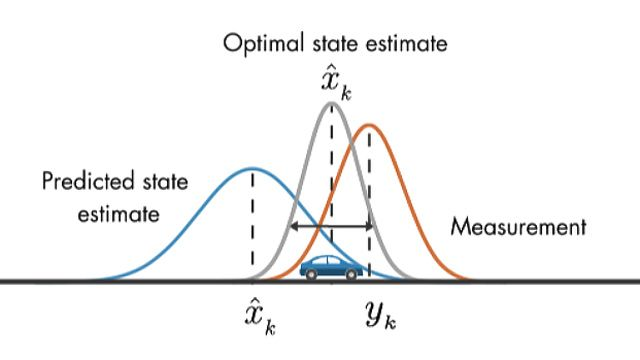
\includegraphics[width=1.0\linewidth]{images/kalman_2.jpg}
    \caption{Kalman filter prediction of the state using estimations. From: \cite{mathworks_kalman}.}
    \label{fig: Kalman filter prediction of the state using estimations.}
\end{figure}
\FloatBarrier\noindent

The Kalman filter follows a classical predict-update model, focusing on a single state variable: the vehicle’s velocity. The process and measurement uncertainty are encapsulated in the following variables:
\begin{itemize}
    \item Process variance Q: models the uncertainty in the vehicle’s motion (e.g., acceleration changes, jitter).
    \item Measurement variance R: represents the uncertainty in each self-speed estimation sample.
\end{itemize}

Where in real life the implementation can be represented as:
\begin{itemize}
    \item Estimated value: the current velocity estimate.
    \item Estimated error: the uncertainty (variance) of the current estimate.
\end{itemize}
At each new frame, a new self-speed estimation is used to update the Kalman filter which effects its output by a variable which is called Kalman Gain 'K':
\begin{equation}
K = \frac{\hat{P}}{\hat{P} + R}
\end{equation}
Where:
\begin{itemize}
    \item $\hat{P}$: predicted error variance
    \item $R$: measurement variance
\end{itemize}
This process allows the filter to balance trust between the incoming measurement and the current estimate. Over time, the filter becomes more confident, reducing the influence of noisy measurements.

Thus, the incorporation of the Kalman filter in this project provides smoother, more reliable self-speed estimation, which enhances the performance of the following dynamic filtering stage.

\begin{figure}[!htbp]
    \centering
    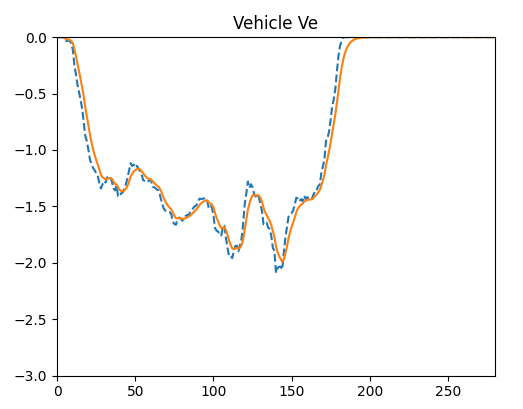
\includegraphics[width=1.0\linewidth]{images/kalman.png}
    \caption{Raw self-speed vs. self-speed after Kalman filter.}
    \label{fig: Test vehicle actual speed vs estimated speed.}
\end{figure}
\subsection{Calculation of $v_{e}$ and $v_{e}$ vs. Self-Speed Filter}

As the emergency braking system should only react to stationary targets, only the points of those targets should be passed to the next stage, the clustering stage.
Filtering out all points that might be invalid or from moving targets ensures a reliable operation of the clustering process and also effectively reduces processing time as a result of the smaller amount of points.
This filtering operation was implemented using a simplistic approach by assuming that theoretically all points of stationary targets should show a velocity equal to the vehicle's velocity when the radar sensor is moving with the vehicle.
By comparing the points' velocities to the prior obtained self-speed, invalid points or those of dynamic targets can be separated and filtered out.
Due to the working principle of radars and the resulting radar sensor's output format, the dependency between the radial speed and the point's angle to the radar sensor must be taken into account.
\par
The whole block was separated into two sub-stages following after each other.
In the first sub-stage, the angle-independent points' speeds, called $v_{e,p}$, are calculated. 
The following sub-stage executes the filtering operation by comparing the points' $v_{e,p}$ to the vehicle's velocity, supplied by the Kalman filter's output.
The calculation of $v_{e,p}$ followed the same approach that was used in the self-speed estimator.
An angle $\phi_{p}$ was defined between each individual point $p$ of the point cloud and the radar sensor's centerline (see \ref{fig:def_angle_phi}).
This angle is calculated for every point by using the prior presented formula.
The dependency between the point's radial speed $v_{r,p}$ and the calculated angle $\phi_{p}$ is then used to calculate each point's angle-independent speed $v_{e,p}$:
\begin{equation*}
    v_{e,p} = \frac{v_{r,p}}{cos(\phi_{p})}
\end{equation*}
A division by zero never occurs because of the first static filtering stage.
Filtering by $v_{e,p}$ is done by calculating the difference between the estimated vehicle's self-speed and $v_{e,p}$ and comparing it against a threshold.
The comparison of the difference to a threshold is needed as $v_{e,p}$ will rarely be exactly equal to the vehicle's self-speed.
A threshold of \SI{0.5}{\meter\per\second} was found out to be sufficient.
After filtering, the points are passed to the clustering stage.

\begin{figure}[!htbp]
\centering
\begin{subfigure}{0.24\textwidth}
  \centering
  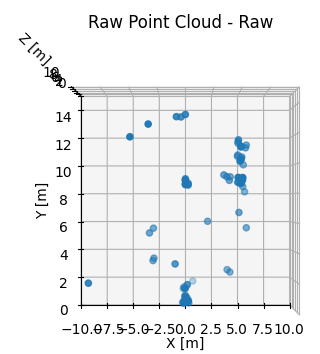
\includegraphics[width=\textwidth]{images/withoutVeFilter.png}
  \caption{Input}
\end{subfigure}
\begin{subfigure}{0.24\textwidth}
  \centering
  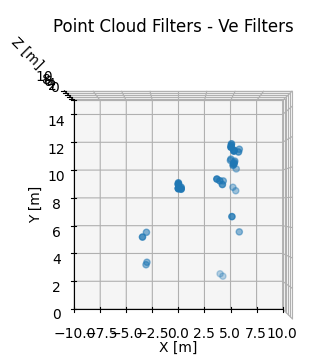
\includegraphics[width=\textwidth]{images/wVeFilter.png}
  \caption{Output}
\end{subfigure}
\caption{Example visualization of the input and output data before and after passing the $v_{e}$ vs. self-speed filtering stage.}
\label{fig:example_ve_filtering_stage}
\end{figure}
\FloatBarrier\noindent

\subsection{Clustering}
Clustering is a fundamental technique used to group similar data points based on their characteristics. It is particularly useful in sensor data analysis for automotive applications, enabling the effective detection and tracking of objects such as vehicles, obstacles, and pedestrians.
\par
Among various clustering algorithms available, DBSCAN (Density-Based Spatial Clustering of Applications with Noise) stands out due to its ability to automatically detect clusters of varying shapes and sizes (see \cite{geeksforgeeks_dbscan}), and to effectively identify and manage noise or outliers. Unlike centroid-based methods such as K-means, which require specifying the number of clusters in advance and struggle with irregularly shaped data, DBSCAN identifies clusters based on the density distribution of data points. Additionally, hierarchical methods like agglomerative clustering, although flexible, tend to be sensitive to noise and computationally expensive for large datasets.

\begin{table}[htbp]
\centering
\resizebox{\columnwidth}{!}{%
\begin{tabular}{|l|l|p{3.5cm}|p{3.5cm}|p{3.5cm}|}
\hline
\textbf{Algorithm} & \textbf{Type} & \textbf{Strengths} & \textbf{Weaknesses} & \textbf{Best Use Case} \\ \hline
DBSCAN & Density-Based & \begin{itemize}
    \item Automatically detects clusters of \textbf{different shapes and sizes}
    \item Identifies \textbf{outliers (noise points)}
\end{itemize} & \begin{itemize}
    \item Computationally expensive for \textbf{large datasets}
\end{itemize} & Radar object detection with noise filtering \\ \hline
K-Means & Centroid-Based & \begin{itemize}
    \item Fast and efficient for \textbf{large datasets}
\end{itemize} & \begin{itemize}
    \item Requires a \textbf{fixed number of clusters (K)}
    \item Struggles with \textbf{irregularly shaped clusters}
\end{itemize} & Segmenting structured radar data with known object counts \\ \hline
Agglomerative & Hierarchical & \begin{itemize}
    \item Does not require specifying number of clusters
    \item Can be modified to detect \textbf{hierarchical structures}
\end{itemize} & \begin{itemize}
    \item Can be \textbf{sensitive to noise}
    \item Computationally expensive for \textbf{large datasets}
\end{itemize} & Grouping similar radar signatures in post-processing \\ \hline
\end{tabular}%
}
\caption{Comparison of Clustering Algorithms}
\label{tab:clustering_algorithms}
\end{table}

For this project, DBSCAN's strengths align closely with the requirements of radar object detection, where the number of detected objects can change dynamically and the presence of noise is common. DBSCAN's capability to handle varying densities and noisy data makes it the optimal choice for accurately and efficiently analyzing real-time radar sensor data in automotive applications.

However, this is insufficient to fully meet the requirements of object detection. It is acknowledged that DBSCAN is among the most efficacious and straightforward instruments available for achieving this objective. However, it is important to note that the sizes of the objects under observation can vary significantly from one frame to the next, and the presence of noise can introduce additional variability. To address these challenges, a two-stage clustering approach was chosen, utilizing DBSCAN as a filter and a clustering algorithm.
The first stage that acts as a filter with DBSCAN parameterized by an Epsilon of \SI{2}{\meter} and a minimum number of samples to specify a core point of 2.
The justification for using it as a filter is that, at first, a broad or permissive set of parameters is applied, making it easier to filter out points or data that are considered as noise. This is not due to the presence of "real" noise; rather, it is owing to a lack of the required amount of points to qualify as an object.
This principle is represented in the next figure:
\begin{figure}[!htbp]
    \centering
    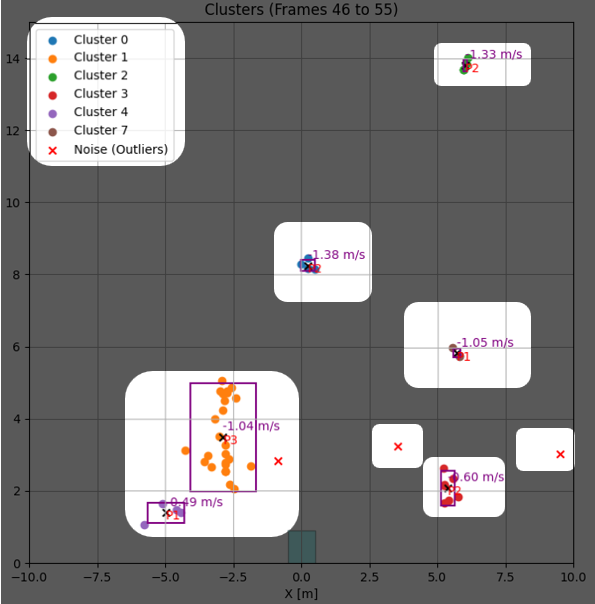
\includegraphics[width=1.0\linewidth]{images/clustering.png}
    \caption{First clustering stage}
    \label{fig: First clustering stage}
\end{figure}
\FloatBarrier\noindent
It can be seen that there are three points that are not included in the clusters and seem to be outliers.
These points might belong to an object, but most likely they are caused by clutter or noise.
As they are not included in clusters after first stage, they are discarded and only the points that are included in clusters are passed to the second stage.
\par
The second stage utilizes DBSCAN with a finer set of parameters.
In this stage, Epsilon was chosen to be equal to \SI{1}{\meter} and the minimum number of samples to specify a core point was set to 4.
This results in finer clusters, preventing objects which are close to each other to be recognized as one single cluster.
The clusters are then passed to the brake controller for final object detection and handling of approaching targets.
\subsection{Brake Controller}

A brake controller is a crucial component in autonomous and assisted driving systems, enabling vehicles to respond intelligently to detected obstacles or hazards.
In this project, a simple yet effective braking mechanism was implemented using a linear controller that calculates a safe stopping distance based on the vehicle's current speed.
The controller assumes a linear relationship between speed and stopping distance, a reasonable approximation under controlled conditions and for the rather lightweight go-kart.
The controller's objective is to ensure that if the vehicle is approaching an obstacle inside an area of interest and potentially getting into contact with it, it activates the brake early enough to stop within a safe distance.
Here, the area of interest is a specified area in front of the go-kart encasing the space where an approaching stationary obstacle could become a hazard to the driver and vehicle.
As the distance which is required to stop the vehicle before getting into contact with the obstacle is proportional to the vehicle's speed, the length of the area of interest is coupled to it.
\par
The brake controller's logic is based on the following variables:
\begin{itemize}
    \item Stopping distance $d_{\text{stop}}(v_{\text{current}})$: Estimates how much distance the vehicle requires to come to a complete stop at the current speed, according to the vehicle specifications.
    \item Output signal $brake\_signal(d_{\text{stop}},d_{\text{target}})$: Generates a binary brake signal (0 or 1) based on whether the stopping distance exceeds the target distance. As the current brake controller simply considers if the brake should be applied or not.
\end{itemize}
The stopping distance is computed relative to a reference speed and stopping distance (default: 40~kph $\rightarrow$ 6~meters), allowing for linear scaling:
\[
d_{\text{stop}}(v_{\text{current}}) = \frac{v_{\text{current}}}{v_{\text{ref}}} \cdot d_{\text{ref}}
\]
If the required stopping distance is greater than or equal to the available distance (measured distance to a detected obstacle), the system triggers full braking:
\[
brake\_signal(d_{\text{stop}},d_{\text{target}}) =
\begin{cases}
1 & \text{if } d_{\text{target}} \leq d_{\text{stop}} \\
0 & \text{otherwise}
\end{cases}
\]

\begin{figure}[!htbp]
    \centering
    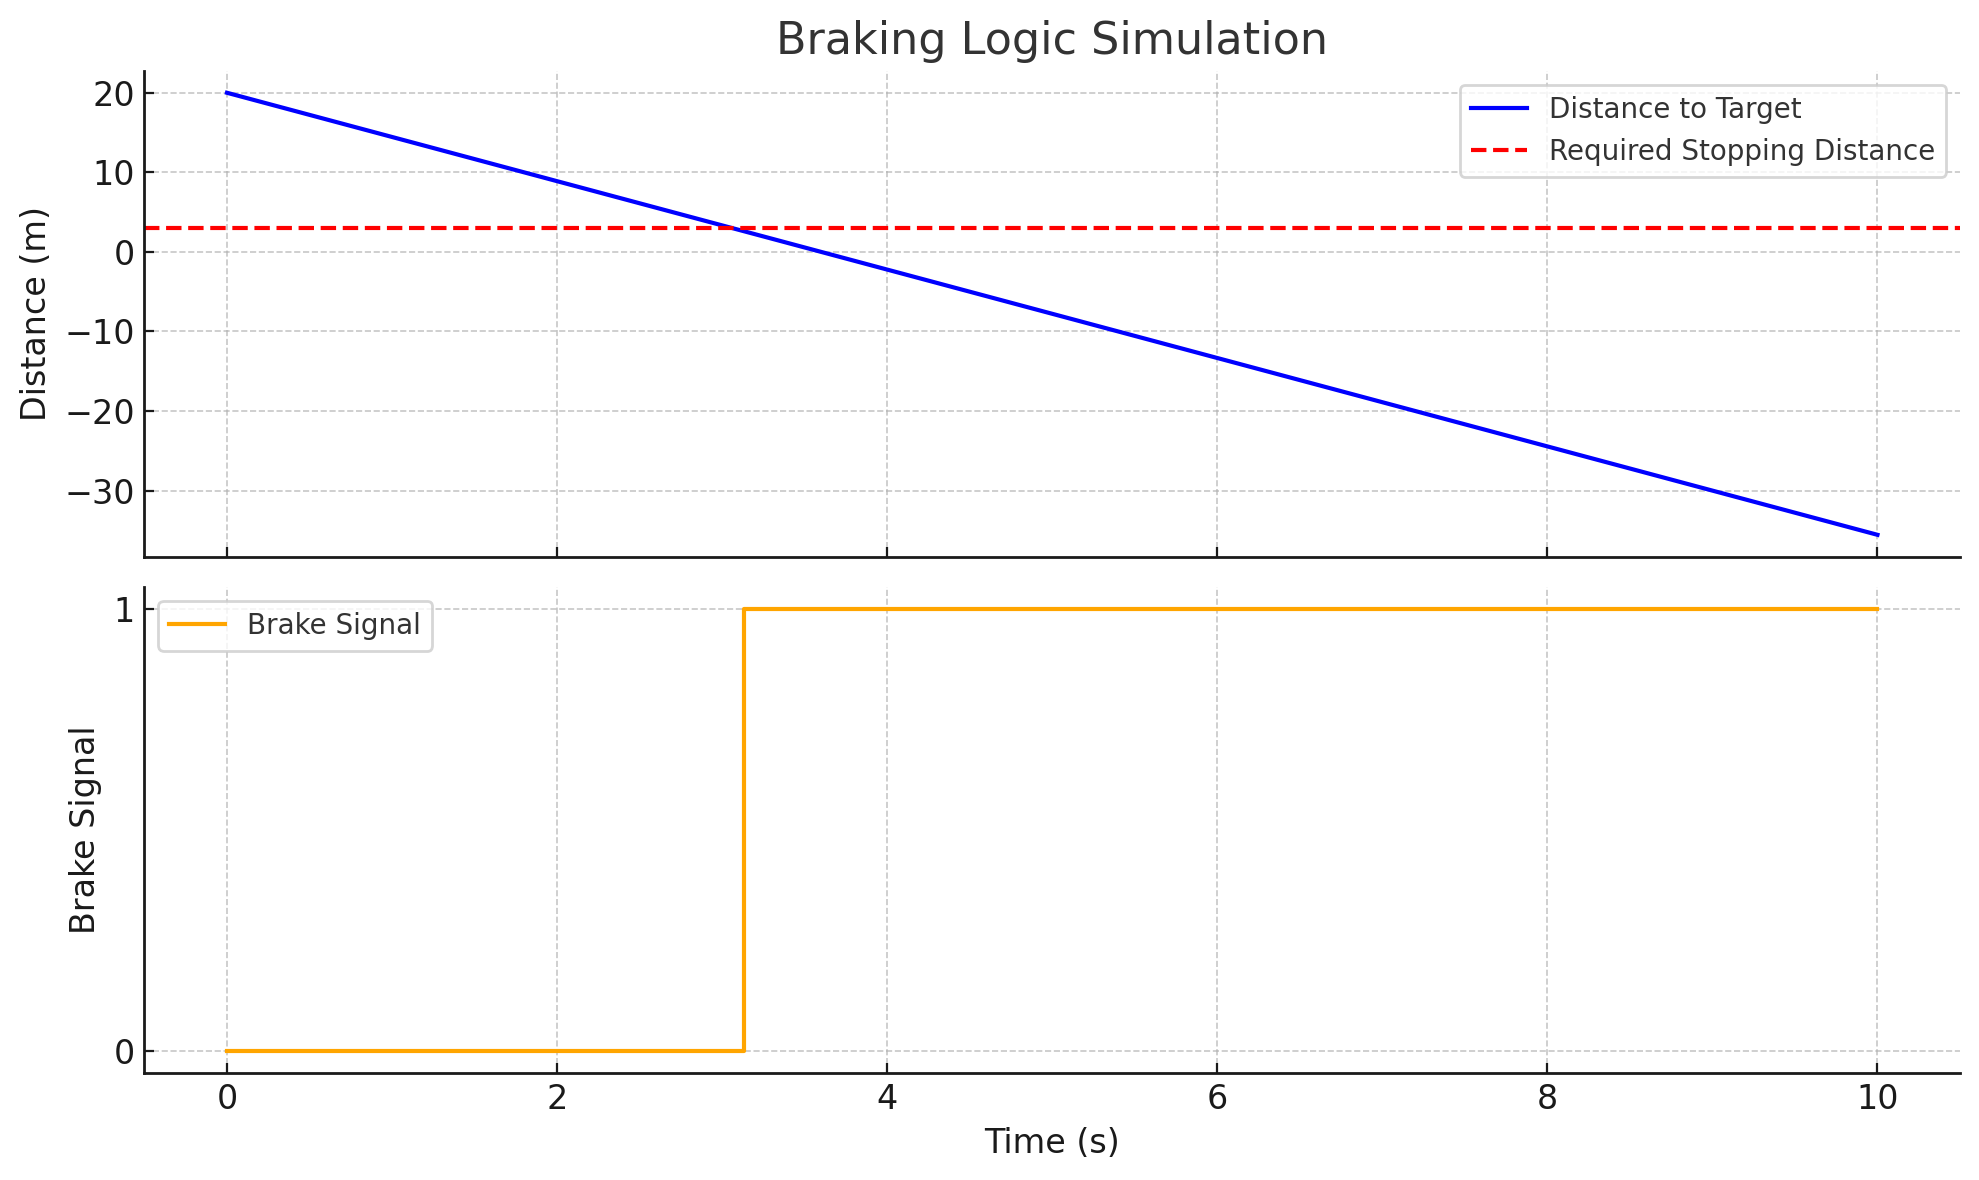
\includegraphics[width=0.8\linewidth]{images/brakeSignal.png}
    \caption{Braking decision based on stopping distance estimation.}
    \label{fig:braking_logic}
\end{figure}
This straightforward logic allows the controller to make quick decisions in real time, helping the vehicle to react safely to moving and stationary objects, detected by the radar.
Although the system is designed to be cautious because it only switches between braking and not braking, it could be improved later by adding smoother braking or more advanced features like adaptive cruise control.
The controller plays a key role in the interaction between detection (from the radar sensor's output data and the processing pipeline) and actuation (braking), forming the basis for a closed-loop safety mechanism.
\section{Summary and Outlook}

% Summary and leasons learned
In this project, an object detection system for a consumer-grade electric go-kart was implemented by using a mmWave radar sensor.
The system successfully meets its primary objectives by accurately detecting obstacles through a custom point-cloud analysis algorithm.
Although the current implementation is limited to stationary objects, it establishes a strong foundation for future development.
All necessary components, including a modular processing pipeline and a hardware interface for safely manipulating the go-kart's brake signal, were developed.
\par
The pipeline's modular architecture proved to support a dynamic developing process, which turned out to be necessary when working with point clouds from radar sensors and an electric go-kart that was not intended to be modified by the end-user.
It also enables further development by expanding, exchanging or modifying processing stages.
During the development, two stages turned out to be extraordinary helpful when it comes to mitigating the influences of the potentially heavily fluctuating point cloud data.
The frame aggregator in combination with running the radar sensor at a high frame rate successfully tackled the problem of data sparsity that sometimes occurred in the test scenario environment.
This was caused by the scenario's "clean" setup without a huge number of targets.
The two-stage clustering approach using the DBSCAN algorithm proved to be able to reliably filter out outliers caused by clutter or noise and was able to provide the brake controller with stable information on stationary objects.
\par
In addition to those two stages, the usage of multiple filtering stages of static and dynamic behavior proved to support the reliability of the whole system.
Static filtering stages early in the pipeline are able to filter out irrelevant points or those with a low level of confidence by using their spatial coordinates and $SNR$ information.
This reduces the required processing time of the later stages by condensing the mass of data to the relevant points.
The dynamic filtering stage allows a reliable differentiation between points that are caused by stationary and moving targets by leveraging the information of the radar-only self-speed estimation.
The approach of using a distance that is linear to the vehicle's velocity to decide whether an emergency braking event should be triggered, and outputting a binary signal, turned out to be sufficient, as the balance board's internal controller prevents the wheels from locking.
\par\bigskip
As with any project, there is always room for improvement, and this work is no exception.
Although the current implementation meets the initial goals and requirements, the algorithm can still be refined.
The project is currently implemented in a threaded solution using Python, which is a result of the dynamic development process where a lot of different techniques and approaches where implemented, tested and sometimes discarded.
Switching from C++, which was used initially used for development, to Python allowed for a quicker development with simpler possibilities of visualization, but also caused a noticeable lack of performance.
This lack of performance showed up in the last stages of development, during testing, and created a delay in the response when tested in an autonomous environment, meaning that when the implementation was not powered by a sufficient power supply, the implemented system showed certain delays in the response when an object was detected in the area for activation of the brake.
It is assumed that the delay originates from Python's heavyweight interpreter and should vanish after porting the system's implementation back to C++.
As for this reason, the decision of not fully merging the existing system into the test vehicle at this stage of the development was made, as it did not provided a fully safe environment for testing.
The validation was done with a LED to indicate the activation of the emergency brake.
An improvement or next step would be to migrate the system back to C++, where the threaded implementation would provide a better response time for each running task.
Further improvements can also be made by incorporating occupancy grids through a Bayesian filter to enhance object detection, allowing the system to go beyond stationary targets.
By improving the system's object detection capabilities to cover moving targets, it would also be possible to estimate their direction of movement, which could significantly improve the driving assistance algorithm and contribute to accident prevention through a more precise analysis.
\par\bigskip
The present status of this project is available in the following GitHub repository: \href{https://github.com/LF-RoGu/Radar-mmWave}{Radar-mmWave on GitHub}.
%\section{WIP - Storing TikZ graphics}

\begin{figure}[!htbp]
    \centering
    \resizebox{0.48\textwidth}{!}{
        \begin{tikzpicture}
            % Block styles
            \tikzstyle{block} = [rectangle, draw, text width=4.5em, text centered, minimum width=6em, minimum height=4em]
            \tikzstyle{block_dashed} = [rectangle, draw, text width=2em, text centered, minimum width=4em, minimum height=4em, dashed]
            % Input and output
            \node[block, right=of antenna, minimum width=4em, minimum height=4em] (frames) {Frames};
            \node[block, right=of frames] (frame_aggr) {Frame\\Aggregator};
            \node[block, right=of frame_aggr] (coord_filter) {Filter\\$x,y,z$\\$\phi,SNR$};
            \node[block, right=of coord_filter] (self_speed_estim) {Self-speed Estimator};
            \node[block, right=of self_speed_estim] (self_speed_kalman) {Kalman Filter};
            \node[block, below=of self_speed_estim] (ve_speed_calc) {Calculation\\of $v_{e}$};
            \node[block, right=of ve_speed_calc] (ve_filter) {Filter\\$v_{e}$ vs. self-speed};
            \node[block, right=of ve_filter] (clustering) {Clustering};
            % Connections
            \draw[->] (frames) -- (frame_aggr); % Connection from antenna to RF amplifier
            \draw[->] (frame_aggr) -- (coord_filter);
            \draw[->] (coord_filter) -- (self_speed_estim);
            \draw[->] (coord_filter.south) |- (ve_speed_calc.west);
            \draw[->] (self_speed_estim) -- (self_speed_kalman);
            \draw[->] (self_speed_kalman) -- (ve_filter);
            \draw[->] (ve_speed_calc) -- (ve_filter);
            \draw[->] (ve_filter) -- (clustering);
        \end{tikzpicture}
    }
    \caption{Block diagram of the pipeline}
    \label{fig:block_diag_pipeline}
\end{figure}

\begin{figure}[!htbp]
    \centering
    \resizebox{0.48\textwidth}{!}{
        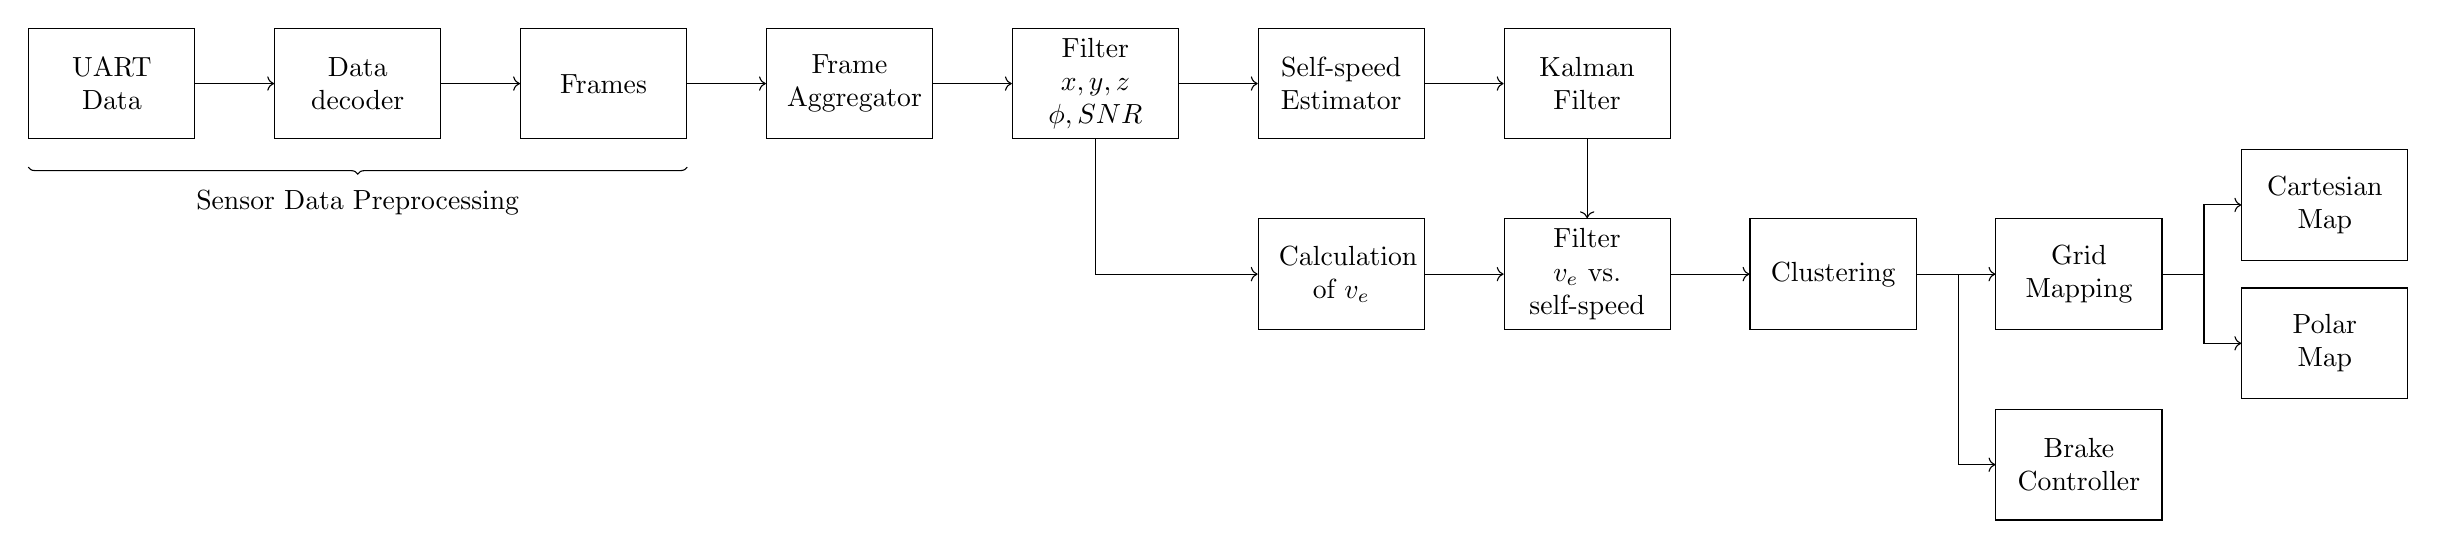
\begin{tikzpicture}
            % Block styles
            \tikzstyle{block} = [rectangle, draw, text width=4.5em, text centered, minimum width=6em, minimum height=4em]
            \tikzstyle{block_dashed} = [rectangle, draw, text width=2em, text centered, minimum width=4em, minimum height=4em, dashed]
            % Input and output
            \node[block] (uart) {UART\\Data};
            \node[block, right=of uart] (decoder) {Data decoder};
            \node[block, right=of decoder] (frames) {Frames};
            \node[block, right=of frames] (frame_aggr) {Frame\\Aggregator};
            \node[block, right=of frame_aggr] (coord_filter) {Filter\\$x,y,z$\\$\phi,SNR$};
            \node[block, right=of coord_filter] (self_speed_estim) {Self-speed Estimator};
            \node[block, right=of self_speed_estim] (self_speed_kalman) {Kalman Filter};
            \node[block, below=of self_speed_estim] (ve_speed_calc) {Calculation\\of $v_{e}$};
            \node[block, right=of ve_speed_calc] (ve_filter) {Filter\\$v_{e}$ vs. self-speed};
            \node[block, right=of ve_filter] (clustering) {Clustering};
            \node[block, right=of clustering] (grid_mapping) {Grid Mapping};
            \node[block, right=of grid_mapping.east, yshift=2.5em] (grid_cartesian) {Cartesian\\Map};
            \node[block, right=of grid_mapping.east, yshift=-2.5em] (grid_polar) {Polar\\Map};
            \node[block, below=of grid_mapping] (brake) {Brake\\Controller};
            % Connections
            \draw[->] (uart) -- (decoder);
            \draw[->] (decoder) -- (frames);
            \draw[->] (frames) -- (frame_aggr); % Connection from antenna to RF amplifier
            \draw[->] (frame_aggr) -- (coord_filter);
            \draw[->] (coord_filter) -- (self_speed_estim);
            \draw[->] (coord_filter.south) |- (ve_speed_calc.west);
            \draw[->] (self_speed_estim) -- (self_speed_kalman);
            \draw[->] (self_speed_kalman) -- (ve_filter);
            \draw[->] (ve_speed_calc) -- (ve_filter);
            \draw[->] (ve_filter) -- (clustering);

            \draw[-] (clustering.east) --++(1.5em, 0) coordinate (arrw_clustering);
            \draw[->] (arrw_clustering) -- (grid_mapping);
             \draw[->] (arrw_clustering) |- (brake);

            \draw[-] (grid_mapping.east) --++(1.5em, 0) coordinate (arrw_mapping_grids);
            \draw[->] (arrw_mapping_grids) |- (grid_cartesian.west);
            \draw[->] (arrw_mapping_grids) |- (grid_polar);

            \draw [decorate, decoration = {brace, mirror, raise=10pt}] (uart.south west) --  (frames.south east) node[pos=0.5,below=15pt,black]{Sensor Data Preprocessing};
        \end{tikzpicture}
    }
    \caption{Block diagram of the pipeline}
    \label{fig:block_diag_pipeline}
\end{figure}


\begin{figure}[!htbp]
    \centering
    \resizebox{0.48\textwidth}{!}{
        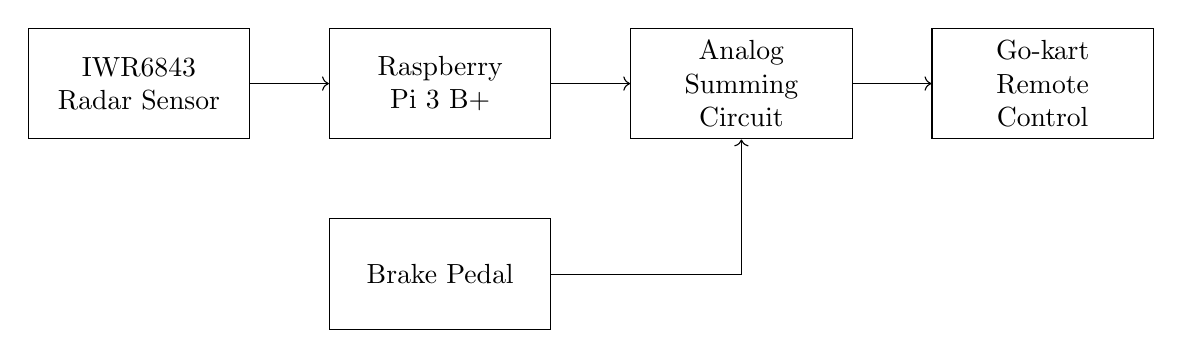
\begin{tikzpicture}
            % Block styles
            \tikzstyle{block} = [rectangle, draw, text width=6.5em, text centered, minimum width=8em, minimum height=4em]
            \tikzstyle{block_dashed} = [rectangle, draw, text width=2em, text centered, minimum width=4em, minimum height=4em, dashed]
            % Input and output
            \node[block] (radar) {IWR6843\\Radar Sensor};
            \node[block, right=of radar] (rpi) {Raspberry\\Pi 3 B+};
            \node[block, right=of rpi] (analog_summ) {Analog Summing\\Circuit};
            \node[block, below=of rpi] (brake_pedal) {Brake Pedal};
            \node[block, right=of analog_summ] (remote) {Go-kart\\Remote Control};
            % Connections
            \draw[->] (radar) -- (rpi);
            \draw[->] (rpi) -- (analog_summ);
            \draw[->] (brake_pedal) -| (analog_summ);
            \draw[->] (analog_summ) -- (remote);
        \end{tikzpicture}
    }
    \caption{Block diagram of the pipeline}
    \label{fig:block_diag_pipeline}
\end{figure}
\newpage

\begin{thebibliography}{00}

\bibitem{ninebot_product_page} Segway Inc., ``Ninebot Go-kart PRO product page'', 2025, Webpage. [Online]. Available: \url{https://de-de.segway.com/products/ninebot-gokart-pro}

\bibitem{iwr_awr_diff} Texas Instruments, ``IWR1642: difference between AWR and IWR parts'', 2025, Webpage. [Online]. Available: \url{https://e2e.ti.com/support/sensors-group/sensors/f/sensors-forum/742730/iwr1642-difference-between-awr-and-iwr-parts}

\bibitem{dev_board_page} Texas Instruments, ``IWR6843AOPEVM product page'', 2025, Webpage. [Online]. Available: \url{https://www.ti.com/tool/IWR6843AOPEVM}

\bibitem{mmwave_demo_doc} Texas Instruments, ``User's Guide mmWave Demo Visualizer,'' 2020, Online Document. [Online]. Available: \url{https://www.ti.com/lit/ug/swru529c/swru529c.pdf?ts=1742817596204}.

\bibitem{understanding_uart} Texas Instruments, ``Understanding UART Data Output Format'', 2025, Webpage. [Online]. Available: \url{https://dev.ti.com/tirex/content/radar_toolbox_2_20_00_05/docs/software_guides/Understanding_UART_Data_Output_Format.html}

\bibitem{mmwave_demo_output} Texas Instruments, ``mmWave Sensing Estimator'', 2025, Webpage. [Online]. Available: \url{https://dev.ti.com/gallery/view/mmwave/mmWaveSensingEstimator/ver/2.5.1/}


\bibitem{ninebot_protocol_github} ub4raf, ``Ninebot-PROTOCOL'', 2025, GitHub Repository. [Online]. Available: \url{https://github.com/ub4raf/Ninebot-PROTOCOL}

\bibitem{ninebot_protocol_scooterhacking} -, ``Ninebot ES Communicaton Protocol'', 2019, Webpage. [Online]. Available: \url{https://cloud.scooterhacking.org/release/nbdoc.pdf}

\bibitem{numpy_polyfit} -, ``numpy.polyfit documentation'', 2025, Webpage. [Online]. Available: \url{https://numpy.org/doc/stable/reference/generated/numpy.polyfit.html}

\bibitem{OccupancyGrid_Mapping_Automotive} Ç. Önen, A. Pandharipande, G. Joseph, and N. J. Myers, ``Occupancy Grid Mapping for Automotive Driving Exploiting Clustered Sparsity,'' \textit{IEEE Sensors Journal}, vol. 24, no. 7, pp. 9240-9250, 2024. [Online]. Available: \url{https://doi.org/10.1109/JSEN.2023.3342463}.

\bibitem{Odometry_radar_only}
D. Casado Herraez, M. Zeller, L. Chang, I. Vizzo, M. Heidingsfeld, and C. Stachniss, 
``Radar-Only Odometry and Mapping for Autonomous Vehicles,'' 
\textit{arXiv preprint}, 2023. [Online]. Available: \url{https://arxiv.org/abs/2305.12409}

\bibitem{EgoMotion_DopplerRadar}
S. R. Bhatt, B. S. Nadiger, R. Parthasarathy, and H. M. Shetty, 
``Instantaneous Ego-motion Estimation Using Doppler Radar,'' 
\textit{IEEE Sensors Letters}, vol. 7, no. 5, pp. 1–4, 2023. [Online]. Available: \url{https://doi.org/10.1109/LSENS.2023.3244030}

\bibitem{Multimodal_Offroad}
C. E. Beal, T. Williams, J. Pauli, M. Mukadam, and B. Boots, 
``Robust Off-Road Autonomy Using Multimodal Sensor Fusion,'' 
in \textit{Proc. of the Conference on Robot Learning (CoRL)}, 2023. [Online]. Available: \url{https://openreview.net/forum?id=kmiZqSgoAt}

\bibitem{HighSpeed_Estimation}
B. Sundaralingam, C. E. Beal, and B. Boots, 
``Robust High-Speed State Estimation for Off-Road Autonomous Vehicles,'' 
in \textit{Proc. of Robotics: Science and Systems (RSS)}, 2023. [Online]. Available: \url{https://openreview.net/forum?id=3JpFLY3ihix}


\bibitem{geeksforgeeks_dbscan}
GeeksforGeeks, 
\emph{DBSCAN Clustering in ML | Density Based Clustering}, 
2023. [Online]. Available: \url{https://www.geeksforgeeks.org/dbscan-clustering-in-ml-density-based-clustering/}. [Accessed: 19-Mar-2025].

\bibitem{mathworks_kalman}
MathWorks,
\textit{Understanding Kalman Filters, Part 3: Optimal State Estimator},
2017. Available at: \url{https://la.mathworks.com/videos/understanding-kalman-filters-part-3-optimal-state-estimator--1490710645421.html} (Accessed: March 23, 2025).

\bibitem{ti_radar_toolbox}
Texas Instruments, 
\textit{Radar Toolbox – mmWave Sensor Configuration and Demos}, 
2024. Available at: \url{https://dev.ti.com/tirex/explore/node?node=A__ADnbI7zK9bSRgZqeAxprvQ__radar_toolbox__1AslXXD__2.20.00.05} (Accessed: March 23, 2025).




\end{thebibliography}


\end{document}
